%%%%%%%%%%%%%%%%%%%%%%%%%%%%%%%%%%%%%%%%%%%%%%%%%%%%%%%%%%%%%%%%%%%
%
%	NOTICE TO COLLABORATORS
%
%	This document is a typeset version of the report on Google Docs. Any content changes
%	should NOT be made in this file, but submitted for review (with tracked changed)
%
%	A few useful commands:
%
%		- \textsc{...} formats text to use small caps. This must be used for acronyms. (eg. EU ETS should be marked up as \textsc{eu ets})
%
%		- \texttt{...} formats text to use monospaced (ie. console like) font. This can be used to any inline references to code
%
%		- For ease of use i have added the \CO command, which can be used to correctly typeset CO2
%
%	Any questions -> cs2309@imperial.ac.uk
%
%%%%%%%%%%%%%%%%%%%%%%%%%%%%%%%%%%%%%%%%%%%%%%%%%%%%%%%%%%%%%%%%%%%

% This is a simple template for a LaTeX document using the "article" class.
% See "book", "report", "letter" for other types of document.

\documentclass[]{article} % use larger type; default would be 10pt

\usepackage[utf8]{inputenc} % set input encoding (not needed with XeLaTeX)

%%% Examples of Article customizations
% These packages are optional, depending whether you want the features they provide.
% See the LaTeX Companion or other references for full information.

%%% PAGE DIMENSIONS
\usepackage{geometry} % to change the page dimensions
\geometry{a4paper} % or letterpaper (US) or a5paper or....
% \geometry{margin=2in} % for example, change the margins to 2 inches all round
% \geometry{landscape} % set up the page for landscape
% read geometry.pdf for detailed page layout information

\usepackage{graphicx} % support the \includegraphics command and options

\usepackage[parfill]{parskip} % Activate to begin paragraphs with an empty line rather than an indent

%%% PACKAGES
\usepackage{booktabs} % for much better looking tables
\usepackage{array} % for better arrays (eg matrices) in maths
\usepackage{paralist} % very flexible & customisable lists (eg. enumerate/itemize, etc.)
\usepackage{verbatim} % adds environment for commenting out blocks of text & for better verbatim
\usepackage{subfig} % make it possible to include more than one captioned figure/table in a single float
\usepackage{cite}
\usepackage{url}
\usepackage{amsmath}
\usepackage{enumitem} %some fancy list stuff
% These packages are all incorporated in the memoir class to one degree or another...

%%% HEADERS & FOOTERS
\usepackage{fancyhdr} % This should be set AFTER setting up the page geometry
\pagestyle{fancy} % options: empty , plain , fancy
\renewcommand{\headrulewidth}{0pt} % customise the layout...
\lhead{}\chead{}\rhead{}
\lfoot{}\cfoot{\thepage}\rfoot{}

%%% SECTION TITLE APPEARANCE
%\usepackage{sectsty}
%\allsectionsfont{\sffamily\mdseries\upshape} % (See the fntguide.pdf for font help)
% (This matches ConTeXt defaults)

%%% ToC (table of contents) APPEARANCE
\usepackage[nottoc,notlof,notlot]{tocbibind} % Put the bibliography in the ToC
\usepackage[titles,subfigure]{tocloft} % Alter the style of the Table of Contents
\renewcommand{\cftsecfont}{\rmfamily\mdseries\upshape}
\renewcommand{\cftsecpagefont}{\rmfamily\mdseries\upshape} % No bold!

\newcommand{\CO}{\textsc{co}$_2$~}

%%% A couple of commands for the title page
\usepackage{hyperref}
\newcommand{\HRule}{\rule{\linewidth}{0.5mm}}

%%% END Article customisations

%%% The "real" document content comes below...

\title{Brief Article}
\author{The Author}
%\date{} % Activate to display a given date or no date (if empty),
% otherwise the current date is printed 

\begin{document}

% BEGIN TITLE AND MESSAGE PAGE
\begin{titlepage}
\begin{center}

% Upper part of the page

\includegraphics[width=0.30\textwidth]{./logo.png}\\[0.45cm]    

\textsc{\LARGE Imperial College London}\\[1cm]
\textsc{\Large Informations Systems Engineering \\ \vspace{5pt} ~}\\[0.5cm]


% Title
\HRule \\[0.4cm]
{ \huge \bfseries Group Project}\\[0.4cm]

\HRule \\[1.5cm]

% Author and supervisor
%\begin{minipage}{\textwidth}
%\begin{flushleft} \large
\textbf{Authors}\\
\vspace{5pt}
\href{mailto:howard.chou09@imperial.ac.uk}{Howard \textsc{Chou}}, 
\href{mailto:thomas.clayson08@imperial.ac.uk}{Thomas \textsc{Clayson}},
\href{mailto:samuel.colliss09@imperial.ac.uk}{Samuel \textsc{Colliss}}, 
\href{mailto:christopher.darby08@imperial.ac.uk}{Christopher \textsc{Darby}}, 
\href{mailto:piotr.dittrich09@imperial.ac.uk}{Piotr \textsc{Dittrich}}, 
\href{mailto:jonathan.ely09@imperial.ac.uk}{Jonathan \textsc{Ely}}, 
\href{mailto:stuart.holland09@imperial.ac.uk}{Stuart \textsc{Holland}}, 
\href{mailto:nicolas.khadivi09@imperial.ac.uk}{Nicolas \textsc{Khadivi}}, 
%\href{mailto:xiaonan.li08@imperial.ac.uk}{Xiaonan \textsc{Li}}, 
\href{mailto:nikunj.patel09@imperial.ac.uk}{Nikunj \textsc{Patel}},
\href{mailto:george.pilikos08@imperial.ac.uk}{George \textsc{Pilikos}}, 
\href{mailto:farhan.rahman09@imperial.ac.uk}{Farhan \textsc{Rahman}}, 
\href{mailto:kanakaratnam.ramanan09@imperial.ac.uk}{Ramanan \textsc{Kanakaratnam}}, 
%\href{mailto:hasanabbas.rehemtulla09@imperial.ac.uk}{Hasanabbas \textsc{Rehemtulla}}, 
\href{mailto:maxwell.revitt09@imperial.ac.uk}{Maxwell \textsc{Revitt}}, 
\href{mailto:chris.socha09@imperial.ac.uk}{Christopher \textsc{Schlumberger-Socha}}, 
\href{mailto:christopher.tory09@imperial.ac.uk}{Christopher \textsc{Tory}}, 
\href{mailto:olivier.van-goethem09@imperial.ac.uk}{Olivier \textsc{van Goethem}}, 
\href{mailto:jonathan.webster08@imperial.ac.uk}{Jonathan \textsc{Webster}}, 
\href{mailto:zipeng.zhou08@imperial.ac.uk}{Zipeng \textsc{Zhou}}, 
\href{mailto:adam.zysko09@imperial.ac.uk}{Adam \textsc{Zysko}} \\ \vfill
%\end{flushleft}
%\end{minipage}
%\begin{minipage}{0.4\textwidth}
%\begin{flushright} \large
\textbf{Supervisor} \\
\vspace{5pt}
\href{mailto:j.pitt@imperial.ac.uk}{Dr Jeremy \textsc{Pitt}}
%\end{flushright}
%\end{minipage}

%\tableofcontents

\vfill

% Bottom of the page
{\large June 2012}

\end{center}
\end{titlepage}


\setcounter{page}{2}

\newpage{}
\thispagestyle{empty}

\vspace*{100pt}
\begin{flushright}
	\textit{It's nice to meet you ladies. Cause we're looking for pussy!}
\end{flushright}

\newpage{}

% END TITLE AND MESSAGE PAGE

\tableofcontents

% \maketitle

\section{Introduction}

At the start of the project, we were introduced to a game consisting of four simple rules:

\begin{enumerate}
\item Each participant is given a number of resources
\item Each participant may put any number of their resources back into a common pool
\item	The resources in the pool are multiplied by a factor N (where $N > 1$)
\item	Each participant may appropriate a given amount
\end{enumerate}

This set of rules describes a very basic Common Pool Resource (\textsc{cpr}) problem. We found that if participants did not follow the rules regarding appropriation, the common pool resource was abused. This led to some participants being left with no resources at all. It was therefore decided that more stringent rules were necessary, where participants could be subject to random monitoring. However, a certain number of resources from the common pool would need to be used to fund this process. The resulting rules were now as follows:

\begin{enumerate}
	\item Each participant is given a number of resources
	\item Each participant must put at least half of their resources into a common pool
	\item The resources in the pool are multiplied by a factor N (where $N > 1$)
	\item Each participant may appropriate a given amount
	\item Participants may choose to monitor others, at the cost of 1 resource being taken from the common pool.
\end{enumerate}

The addition of monitoring led to a more effective prevention of `cheating', and therefore a more efficient distribution of the resource. Indeed, this is a good example of the efficacy of common pool resource utilisation when participants act as individuals, and participants agree on rules and monitoring as a collective.

This report details the research, design, and implementation of a multi-agent simulation of the Kyoto common pool resource system, which is similar to the simple game described above. A multi-agent system is a paradigm for expressing systems composed of intelligent agents acting within a defined environment. This maps well to the Kyoto Protocol, allowing us to simulate individual countries and their governments' attitudes as independent agents. The common pool involved in our model is that of worldwide greenhouse gas (\textsc{ghg}) emissions.

We define our model in greater depth, describing how we build upon the existing architecture of Presage2, a multi-agent simulation engine. After giving an overview of our primary design decisions, we outline the specific implementation of individual components within our simulation. Following this, we present simulation data attained from running our Kyoto Protocol system, and compare how our system performs when compared to reality, as well as what predictions it makes about the long term impacts of the Kyoto Protocol on global emissions.

% What is out of scope in this report


\section{Research}
\subsection{Climate Change}
The consensus among scientists is that the Earth is unequivocally warming, with a high certainty that this is being caused by human activities, specifically due to the last 150 years of industrial development. The International Panel on Climate Change (\textsc{ipcc}) defines climate change as:

\begin{quote}
``A change in the state of the climate that can be identified (e.g. using statistical tests) by changes in the mean and/or the variability of its properties, and that persists for an extended period, typically decades or longer. [\ldots]any change in climate over time, whether due to natural variability or as a result of human activity''~\cite{IPCC-synthesis-07}
\end{quote}

This differs from the United Nations Framework Convention on Climate Change (\textsc{unfccc}) definition, which places the blame more squarely on human cause, where:

\begin{quote}
``[\ldots] climate change refers to a change of climate that is attributed directly or indirectly to human activity that alters the composition of the global atmosphere and that is in addition to natural climate variability observed over comparable time periods.''~\cite{IPCC-synthesis-07}
\end{quote}

There are many different responses to climate change, most focusing on either mitigation (``implementing policies to reduce \textsc{ghg} emissions and enhance sinks'')~\cite{IPCC-glossary-mitigation} or adaptation. (``Initiatives and measures to reduce the vulnerability of natural and human systems against actual or expected climate change effects. Various types of adaptation exist, e.g. anticipatory and reactive, private and public, and autonomous and planned.'')~\cite{IPCC-glossary-adaptation}

\subsubsection{United Nations Framework Convention on Climate Change}

The United Nations Framework Convention on Climate Change (\textsc{unfccc}) is an international environmental treaty which covers most of the countries in the world. It was signed in 1992 with the aim to stabilise the concentration of greenhouse gases (\textsc{ghg}) in the atmosphere ``at a level that would prevent dangerous anthropogenic (i.e. human) interference with the climate system.''~\cite{IPCC-synthesis-01-question1}

The definition of `dangerous' is up to interpretation, although the \textsc{ipcc} concluded that the definition would vary between different regions of the world, primarily dependent on the local consequences of global warming, the region's ability to adapt to climate change and the ability to reduce \textsc{ghg}. Figure~\ref{fig:burning_embers} shows the commonly named `burning embers' diagram, which represents conceptual impact across five ``reasons for concern.''

\begin{figure}[h!]
	\centering
	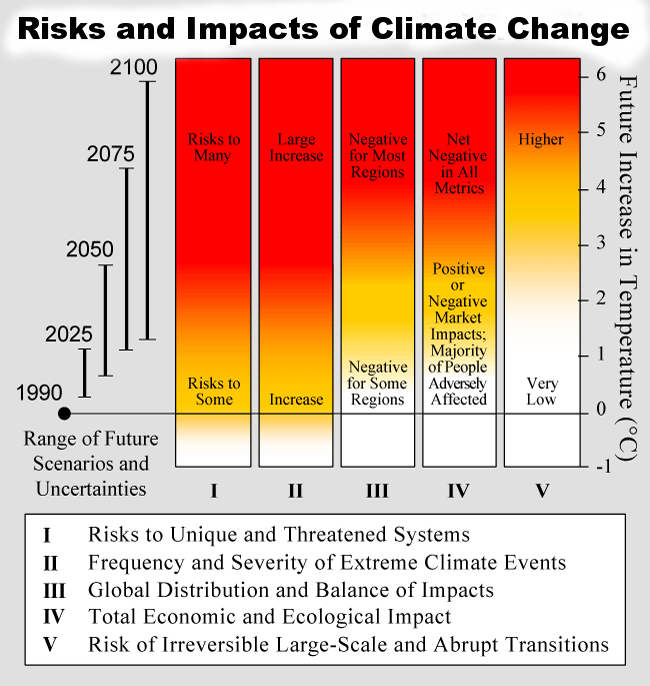
\includegraphics[width=0.6\textwidth]{img/Risks_and_Impacts_of_Global_Warming.png}
	\caption{`Burning embers' diagram~\cite{IPCC-workinggroup-01}}
	\label{fig:burning_embers}
\end{figure}

\subsection{The Kyoto Protocol}

Having recognised that developed countries are primarily responsible for the high levels of \textsc{ghg}s in the atmosphere, the \textsc{unfccc} formed the Kyoto Protocol to not only encourage countries to reduce emissions, but to commit to that reduction.~\cite{UNFCCC-kyoto-summary}To make the Protocol more appealing, carbon taxation was avoided in favour of other carbon reduction mechanisms. 

The initial agreement was signed on the 11th December 1997 during the 3rd annual \textsc{unfccc} conference and then came into force on the 16th February 2005. The Protocol sets mandatory targets on \textsc{ghg} emissions for the world's leading economies ``with a view to reducing their overall emissions of such gases by at least 5 percent below existing 1990 level in the commitment period 2008 to 2012.''~\cite{UNFCCC-98-p1}. Future targets are expected to be drawn up for ``commitment periods'' after 2012.~\cite{UNFCCC-98-p4}

As of September 2011, 191 countries have ratified the treaty with the United States remaining as the only signatory not to have ratified the protocol. However, some United Nation member states such as Afghanistan, Andorra, and South Sudan never signed the agreement and Canada left in December 2011.

The aim of the Kyoto Protocol is to contain emissions of anthropogenic \textsc{ghg}s in a way that reflects underlying national differences in emissions, wealth, and capacity for reduction; this concept is known as ``common but differentiated responsibilities.''~\cite{Grubb-04}\cite{UNFCCC-92} It was recognised that much of the existing \CO emissions were due to developed countries, and that the needs of developing countries would need to be taken into account when calculating emission targets. It was agreed that the per capita emissions of developing countries was still relatively low, and that these participants would be allowed to grow to meet their socio-economic needs.

Participants in the Kyoto Protocol were classified into three groups, according to their responsibilities:~\cite{UNFCCC-92}

\begin{description}
	\item[Annex I] \hfill \\
	Industrialised countries and economies in transition. These countries have committed to reduce their emissions levels of greenhouse gases to targets that are set according to their 1990 emissions.
	
	\item[Annex II] \hfill \\
	Developed countries. Annex II countries are a subset of Annex I countries, and are encouraged to invest in developing countries.

	\item[Non-Annex I] \hfill \\
	Developing countries which are not required to reduce emission levels unless developed countries have supplied funding and technology through outsourcing. This serves three purposes:
	\begin{itemize}
		\item To avoid restricting a country's development, since burgeoning economies tend to rely on carbon based industry.
		\item To permit sale of excess emission capacity to those nations having difficulty meeting their targets.
		\item To encourage investment from Annex I countries in low-carbon technology.
	\end{itemize}
\end{description}

The Protocol structures rolling emission reduction commitment periods, with the first scheduled to end in 2012.

\subsubsection{Initial Commitment Period}

Parties partaking in the Kyoto Protocol commit themselves to reducing four \textsc{ghg}s (carbon dioxide, methane, nitrous oxide, and sulphur hexafluoride) and two other groups of gases (hydrofluorocarbons and perfluorocarbons). These are considered \CO equivalents when calculating emission reduction.

With the understanding that only Annex I countries have targets that they must commit to, the aim is to reduce global \CO emissions to at least 5\% below the base year by the end of the first commitment period. Through negotiation, the base year decided on was 1990, due to the lack of accurate data for years prior to this. Participants would need to agree to their individual targets in line with the global target, the results of which can be seen in Table X. It should be noted that the \textsc{eu}-15 opted for a `burden sharing agreement' whereby the \textsc{eu} set a target of -8\%, and assigned individual targets to its member states.

[TABLE]

Countries can meet their targets by reducing their greenhouse gas output or by offsetting their output by using the flexible mechanisms outlined in the Protocol. Even if Annex I countries meet their targets for the first period, future reductions will be required if the overall goal of \textsc{ghg} stabilisation is to become a reality.

\subsubsection{Flexible Mechanisms}

While participant countries must meet their emission targets primarily through domestic carbon reduction methods, Flexible Mechanisms were also put in place to make targets more attainable and affordable. These market based mechanisms help stimulate sustainable development through technology transfer, help countries with Kyoto commitments to meet their targets in a cost-effective way, and encourage the private sector and developing countries to contribute to emissions reduction. The three mechanisms defined in the Protocol are:

\begin{description}
	\item[Emissions Trading] \hfill \\
	Member states can trade a newly created commodity representing the surplus created if their emissions are below their assigned target.
	
	\item[Clean Development Mechanisms] \hfill \\
	Annex I \& II countries can invest in sustainable, greenhouse gas reduction projects in Non-Annex countries in exchange for `Certified Emission Reductions' (\textsc{cer}).~\cite{UNFCCC-05}

	\item[Joint Implementation] \hfill \\
	Annex I countries can invest in sustainable greenhouse gas reduction projects in other Annex I countries as an alternative to national reduction.
\end{description}

\paragraph{International Emissions Trading}

With international markets already trading in commodities, Article 17 of the Protocol allows for countries to sell their excess `Assigned Amount Units' (\textsc{aau}s) to countries unable to meet their target. This ability for countries to sell their excess capacity saw the birth of the `carbon market'.

Some Annex I countries, categorised as Economies In Transition (\textsc{eit}), have a large surplus of \textsc{aau}s, which can be sold on the carbon market. One example is Russia: having closed many cold-war-era industries since its 1990 base year, Russia was given more headroom for growth when its carbon target was set. Despite the abundance of \textsc{aau}s in the market, to stop countries overselling units and becoming unable to meet their own targets, participants must keep a reserve of \textsc{aau}s (known as a `commitment period reserve') which cannot fall below 90\% of its assigned amount.

\subparagraph{European Union Emission Trading System}

The European Union Emission Trading System (\textsc{eu ets}) allows for trading between participants in the EU and between industry operators in the \textsc{eu}. Governments of \textsc{eu} states agree on national emissions caps, and then allocate allowances to their industrial operators. Operators may privately move allowances between themselves, privately match buyers and sellers, or trade on the carbon exchange. Trading has proved to be very unpopular outside of the \textsc{eu}.~\cite{Grubb-09}

\paragraph{Clean Development Mechanisms}

Article 12 of the Protocol allows for Clean Development Mechanisms (\textsc{cdm}), whereby Annex I countries may invest in emission-reducing projects in developing countries. In exchange, projects earn saleable \textsc{cer} credits, which the investor may use to meet their target. Article 12 of the Protocol describes its objectives:

\begin{itemize}
	\item Assist Annex I parties to develop sustainable emission-reduction projects in Non-Annex countries (in line with the primary \textsc{unfccc} goal).
	\item Assist Annex I parties to meet their emission targets.
\end{itemize}

Figure~\ref{fig:cdm_map} shows a map of \textsc{cdm} projects worldwide.

\begin{figure}[h!]
	\centering
	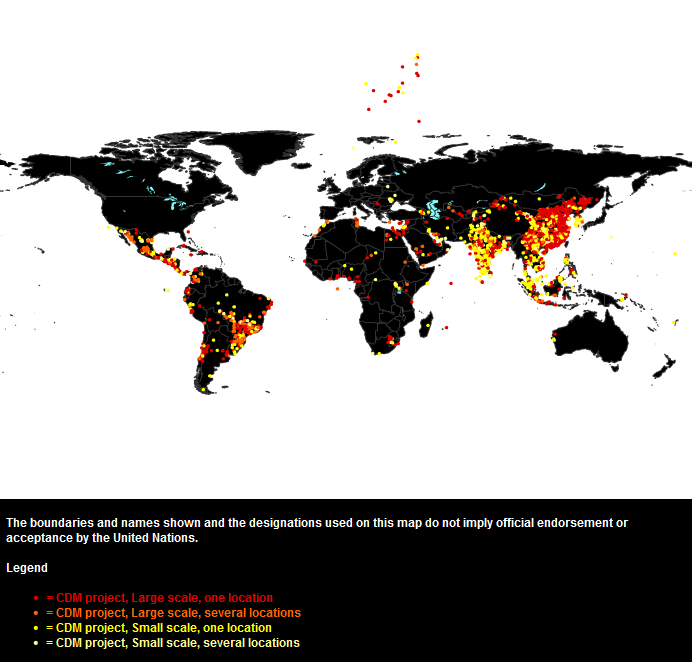
\includegraphics[width=0.8\textwidth]{img/CDM_Map.png}
	\caption{Map of \textsc{cdm} projects worldwide~\cite{UNFCCC-CDM-map}}
	\label{fig:cdm_map}
\end{figure}

Industrialised countries wishing to take part in \textsc{cdm} need to get assurance from the project host that it will contribute to sustainable development. The applicant must also prove that the project would not have happened regardless of their support, and must project future emissions had the project not gone forward. This ensured there are no `free riders' and that the applicant is awarded the correct amount of units for their contribution to the project.

\paragraph{Joint Implementation}

Article 6 defines the Joint Implementation (\textsc{ji}) mechanism, which allows countries to invest in carbon-reduction projects in other Annex I countries as an alternative to national emission reduction. In exchange for the investment, the investor will be awarded an Emission Reduction Unit (\textsc{eru}), which is to be taken from the investee's \textsc{aau} pool. This requirement ensures that the total amount of units shared between Annex I countries does not change during a commitment period.

\textsc{ji} may be advantageous where carbon reduction is cheaper to implement in another Annex I country rather than nationally (an example might involve replacing dirty power plants with cleaner energy producers). To date, \textsc{ji} has not been very popular, with only 22 projects having been registered prior to 2008. %citation needed

\subsubsection{Reporting, Monitoring and Sanctioning}

Each participant must designate an authority to create and manage its \textsc{ghg} inventory. While not specifically required, many non-annex countries have also set up national bodies to manage their Kyoto obligations (primarily \textsc{cdm}s).

Kyoto requires that:~\cite{UNFCCC-Kyoto-guidelines}

\begin{itemize}
	\item Annex I countries must have in place a national system to estimate \textsc{ghg} emissions (natural and anthropogenic) and any \CO that has been removed through sinks.
	\item Annex I countries must report their greenhouse inventories annually and provide regular communication detailing supplementary information to demonstrate compliance.
	\item Expert review teams periodically review greenhouse inventories and any national communications (this must be conducted at least once every 5 years).
\end{itemize}

The efficacy of the Kyoto Protocol depends on the participants following the Protocol's rules and regulations with respect to their commitments and the accuracy and reliability of their reports. Keeping in line with the core aim of the Kyoto Protocol (that is, an alternative to a carbon tax) financial sanctions were avoided, instead opting for the setting of harsher emissions targets.

Part of monitoring involves an expert review of reports submitted by participants. Reviewers may mark reports as `question of implementation' where there is an unresolved problem regarding implementation, may suggest `adjustment' where inventory is incomplete, and may suggest `correction' where there are clear inconsistencies (suggesting `cheating'). `Correction' is analogous to an inventory adjustment.~\cite{UNFCCC-reporting-review}

There are also sanctions for parties not meeting the emissions target they committed to. If the enforcement branch determines that Annex I countries do not comply with their emissions limitations, that country is required to make up the difference in future commitment periods plus an additional 30\%. That country will also be suspended from emissions trading.~\cite{UNFCCC-compliance}

\subsubsection{Criticisms}

Opinions on the effectiveness of the Kyoto Protocol vary significantly; while some consider it a move in the right direction for the stabilisation of \textsc{ghg} emissions, others believe the Protocol is inherently unfair and ineffective.

\paragraph{Inception}
Problems of fairness were raised early in the negotiation stages of the Protocol. During the negotiations for the setting of the base year, 1990 was chosen as reliable data prior to this date was unavailable. This base year was also highly favoured by the \textsc{uk}, Germany, and Russia as their respective \CO levels were high in 1990. Following 1990, \textsc{uk} emissions dropped as the energy sector moved away from coal power, toward cleaner gas power stations. Germany's \CO emissions also decreased following 1990 when East Germany and West Germany reunited, resulting in a decrease in dirty industry in East German territories. There was much disagreement as Japan wished to use 1995 as the base year, while former Soviet block countries wanted to use emission rates from before their industrial collapse at the end of the cold war.

There were also disagreements over the size of the emission cuts, with the \textsc{eu} supporting cuts in the range of 10-15\%, while the \textsc{us} wanted a more conservative cut of between 0-5\%. The level of cutbacks wanted varied from country to country, with the only common theme being that the proposals suited the interests of the country making the proposal.~\cite{Grubb-economics}

\paragraph{Trading}
There was also concern regarding the implementation of emissions trading. The \textsc{eu} and Japan wanted to ensure that emission trading was free and transparent, and wanted to prevent the \textsc{us} from using its political pressure to gain preference when trading with Russia. This concern was echoed in developing countries, where they believed the \textsc{us} would use flexibility mechanisms to its own advantage, over the interests of less able countries that needed support.

With Russia having an abundance of \textsc{aau}s, there was concern that it would have a monopoly on the carbon trading market, and would be able to adversely affect the price of carbon. Russia could withhold \textsc{aau}s to inflate the price for units, and inflate its profits. While possible, the situation was also difficult for Russia, since it has both an excess of \textsc{aau}s, and was one of the largest oil producers. Selling \textsc{aau}s would encourage the purchasing of oil, while withholding \textsc{aau}s would increase their value, but might adversely affect the price of fossil fuels.

\paragraph{The effect of Non-Annex countries}

Following successful negotiation and signing of the Protocol, concern was raised regarding the lack of limitations on the \textsc{ghg} emissions of developing countries. Indeed the \textsc{us} did not ratify the Protocol, stating that ``it exempts 80\% of the world, including major population centers such as China and India, from compliance, and would cause serious harm to the \textsc{us} economy''.~\cite{Hague-to-Marrakesh} Statistics from the International Energy Agency (\textsc{iea}) show by 2011, emissions from Non-Annex I countries had exceeded those from Annex I countries.~\cite{IEA-highlights} Only 3 countries from the top 10 table of carbon emitters are currently an Annex I participants.

\subsection{Common Pool Resources}

A Common Pool Resource (\textsc{cpr}) is a natural or man-made resource in which: the resource is deductible; the size and characteristic of the resource make it difficult to exclude other from its use.~\cite{Ostrom-90} \textsc{cpr}s are defined by their core resource (\emph{stock variable}) and the limited quantity of extractable units (\emph{flow variable}). The stock variable is to be conserved such that consumers may continue to exploit/consume excess resources (\emph{fringe variable}), which are produced at a rate defined by the flow variable.

Due to a \textsc{cpr}'s deductible, non-exclusive characteristics; it may suffer from congestion or overuse. Many \textsc{cpr} systems form positive feedback loops, and so with careful resource management (ensuring the stock variable is not compromised), fringe units will be continually produced, allowing for efficient operation. Excessive consumption (consumption exceeding the flow variable) will reduce the stock variable, which in turn will reduce the flow variable. Unless the stock variable is allowed to regenerate, excessive use will result in resource depletion; even if the stock is allowed to regenerate, the damage may be irreparable. The key to efficient \textsc{cpr} is to ensure the resource is not abused.

An example of \textsc{cpr} is commercial fishing; by overfishing certain species of fish, the stock variable (number of fish) is reduced, which in turn reduces the flow variable (birth rate), which decreases the fringe units which can be sustainably caught by fishers. Unless the stock variable is allowed to regenerate, certain species of fish may be driven to depletion (extinction). This is an example of inefficient use of a \textsc{cpr}, the only viable solution to which is drastically reducing the rate of fishing. This, and further example cases, are discussed in more detail later.

While some \textsc{cpr}s are owned by governments or private parties, making these public or private goods, many have no ownership, and so are an open access resource. We should note the difference between `Common Pool Resources', as described above, and `The Commons', which

\begin{quote}
	``refer to systems, such as knowledge and the digital world, in which it is difficult to limit access, but one person's use does not subtract a finite quantity from another's use.''~\cite{Ostrom-challenge-90}
\end{quote}

With the understanding that uncontrolled access to a \textsc{cpr} will lead to inefficiencies and overuse, some resource consumers form an institution, often called a `Common Property Regime', to reduce the threat to the common resource by independent actions and increase the efficiency of resource harvesting.

\subsubsection{Common Property Regime}

Common Property Regimes are formed to protect and maintain resource systems by coordinating strategy. These strategies are based on the protection of the core resource, with fringe units being allocated to participants based on an arranged scheme. While regimes can be effective at protecting \textsc{cpr}s, the difficulty is in the devising of rules, limits, sanctions, and other operational variables.

The correct setting of appropriation limits is important, as setting limits too low could lead to overuse and eventual depletion of the resource, conversely setting limits too high reduces the efficiency at which the resources can be harvested. In Common Property Regimes, access to the common property is no longer free; those outside the regime see the resource as a private good, while those part of the regime see it as common good (albeit one in which appropriation is carefully monitored.)

Elinor Ostrom defined eight design principles which are required for an effective Common Property Regime:~\cite{Ostrom-90}

\begin{itemize}
	\item Clearly defined boundaries
	\item Congruence between appropriation and provision rules and local conditions
	\item Collective choice arrangements allowing for the participation of most of the appropriators in the decision making process
	\item Effective monitoring by monitors who are part of or accountable to the appropriators
	\item Graduated sanctions for appropriators who do not respect community rules
	\item Conflict-resolution mechanisms which are cheap and easy of access
	\item Minimal recognition of rights to organize (e.g. by the government)
	\item In case of larger \textsc{cpr}s: Organisation in the form of multiple layers of nested enterprises, with small, local \textsc{cpr}s at their bases
\end{itemize}

Indeed Ostrom continues to say:

\begin{quote}
	``When subjects are placed in settings in which decisions are made in isolation, with minimal institutional structure, their aggregate behaviour is generally consistent with equilibrium predictions of inefficient resource use. On the other hand, when allowed to communicate or use other coordinating mechanisms, subjects often adopt and maintain agreements consistent with efficient and sustainable resource use''~\cite{Ostrom-rules}
\end{quote}

\subsubsection{Case Study}

These case studies look at examples of \textsc{cpr}s in the real world, the strategy behind these, and whether theses are considered a success.

\paragraph{Commercial fishing}

The fishing industry currently generates in excess of 80 billion \textsc{usd} every year, but it is an industry in danger due to the diminishing supply of commercially viable fish caused by overfishing. In 1979, it was believed that with existing conventional fishing practices, the growth era of fisheries was over.

While this estimate was not totally accurate (the fishing industry is still growing), the problem of overfishing has also continued to grow. As briefly described in an earlier section, by overfishing certain species of fish, the stock variable (number of fish) is reduced, which in turn reduces the flow variable (birth rate), which decreases the fringe units which can be sustainably caught by fishers. Unless the stock variable is allowed to regenerate, certain species of fish may be driven to depletion (extinction).

Some believe this problem is caused by lack of property rights for fish species in the ocean, and so tried to come up a solution which impart property rights which could then be controlled and regulated. In 1982, the United Nations Conference on the Law of the Sea established Exclusive Economic Zones (\textsc{eez}s) which were assigned to countries with coastal region, with the aim of regulating fishing and reducing overfishing.~\cite{Canada-sea-law}

``[\ldots]not only do governments now have the legal power and the self-interest to apply sound principles of resource management within this area, but they have an obligation to do so.''

Instead of imposing restrictions on fishing, many countries expanded their fishing fleets to take advantage of their new `property'. This was due to incorrect data and models used by various countries when calculating what limitations would need to be put in place, which indicated an increase was feasible.

\paragraph{Ozone Layer \& CFCs}

Scientists in the 1970s discovered an area of the Antarctic stratosphere with very low levels of ozone (33\% less than ozone level for that area pre-1975), which became known as the ozone hole. This ozone layer depletion would lead to increased \textsc{uv} levels passing through the ozone layer, which was a concern in the short term due to the increased risk of skin cancer and a concern in the long term as it could have a catastrophic effect on the biosphere. Indeed these holes were expanding, with the hole over the south pole covering most of the Antarctic.

Chlorofluorocarbons (\textsc{cfc}s) were to blame for this destruction of the ozone layer, with a single \textsc{cfc} molecule having the power to chemically unbind 4000 molecules of the ozone.~\cite{Canada-sea-law} In this instance, the flow variable is the natural production of ozone (produced by short wave \textsc{uv} rays reacting with oxygen); while the compromising of the stock variable was not a problem (ozone will always be naturally produced), the effect of us destroying the fringe units would have a catastrophic effect upon our lives, and so would need to be conserved. The solution to this was a proportional cutback of 100\%, which would put us on the right track to stop the ozone hole increasing in size, and eventually would lead to a decrease in size.

A regime was put in place, the `Montreal Protocol on Substances that Deplete the Ozone Layer', which was adopted by 125 countries in 1987 and planned to cut production of \textsc{cfc}s over 10 years. This would be expensive for propellant and refrigeration industries, substantially increasing the cost to manufacture these products for both producers and consumers.

The ozone holes have ceased growing (and will eventually disappear), and so this example case of \textsc{cpr} can be considered a success. While the required actions were expensive for the \textsc{cfc} industry, the benefits for humanity far outweigh the losses to that industry.

\paragraph{Analysis}

The success of schemes to protect \textsc{cpr}s worldwide varies substantially. The key to success is understanding that there is no `one-size-fits-all' solution to the problem of common resources, and that often quick fixes can cause more harm than good. While Ostrom's design principles are an integral part of Common Property Regimes, studies on the relative successes of \textsc{cpr} implementation has shown that there are a few requirements for a successful regime:~\cite{Ostrom-challenge-90}

\begin{description}
	\item[Achieving accurate and relevant information] \hfill \\
	Published information must combine accurate scientific data with an understanding of the environmental system. With the continually evolving environment, data must be kept up to date so that it is relevant. 
	
	\item[Dealing with conflict] \hfill \\
	When resources are allocated, conflict over policy and administration of regime will certainly occur. Conflicts should not be ignored, but dealt with immediately to ensure these do not become a problem further down the line. 

	\item[Enhancing rule compliance] \hfill \\
	Rules are only effective when participants consider these legitimate, fair and enforced. Participants should take some responsibility for monitoring.
	
	\item[Providing infrastructure] \hfill \\
	Physical, technological, and institutional infrastructures must be provided such that participants may operate effectively within the regime
	
	\item[Encourage adaptation and change] \hfill \\
	It is difficult to `fix' institutions for the long term, when they are still dealing with past issues. Institutions must embrace changes as part of their developments.
\end{description}

\subsubsection{The Kyoto Protocol as a CPR}

The problem which the Kyoto Protocol attempts to resolve, the reduction and stabilisation of global carbon emissions, is not dissimilar to other \textsc{cpr} problems already discussed in this report. Both the Kyoto Protocol and \textsc{cfc} reductions are \text{cpr} systems which have a global effect on the environment, economies, and development. The difference between these problems however, is one of scale.

In the first instance, Kyoto is an open resource with no real ownership; this makes it difficult to impose regulations and limitations on emissions, even if a Common Property Regime is formed. Unlike the \textsc{cpr} system involving fisheries, dividing up the world’s atmosphere by country does not prevent the actions of other adversely affecting the global environment, and unlike the problem of \textsc{cfc}s, the economic consequences are large and affect the development of countries, not just individual industries.

As in the overfishing example, participants will always attempt to play to their advantage. We have seen this to be the case in Kyoto, as described in the Criticisms subsection of the report, and this may lead to inefficiencies within the Kyoto \textsc{cpr} system. While the long term gains from participating in the Protocol are obvious, some have more to gain than others, particularly in the short term. Russia, with its excess of \textsc{aau}s has the potential to make money on the emissions trading system (or indeed, play with the market to increase profits).

The \textsc{eu}, having seen the efficiency advantages of working as part of a common regime, have further imposed regulations, systems, and sanctions within the member states. The aim of this is to ensure \textsc{eu} members are as efficient as possible within the scope of the \textsc{cpr}. Indeed this appears to be the case, as most \textsc{eu} states are on track to meet their target.~\cite{EEA-Tracking-progress-20}

Research has also shown that there may be problems of efficiency when there are significant wealth and technology inequalities. Where there are no regulations for a \textsc{cpr}, technology inequalities can exacerbate inefficient use and those participants with better technologies over-extract from the core resource, while less technologically advanced participants will lag behind. Where \textsc{cpr}s are regulated, efficiency gains from  the regime will be lower as inequality amongst participants increases. This has somewhat been avoided in the Kyoto Protocol by the introduction of Clean Development Mechanisms; this allows Annex I countries to invest in clean development in Non-Annex countries, thereby reducing the technology gap between developing and developed countries, which in turn increases the efficiency of participants in this regime.~\cite{Wealth-inequality-regulated}\cite{Wealth-inequality-unregulated}

\paragraph{Summary} It appears that Kyoto can be mapped to a Common Pool Resource scheme, and while some of the problems faced by other \textsc{cpr} systems have been carefully thought out (efficiency of regimes, \textsc{cdm} to combat wealth inequality), other problems still remain (no limits for Non-Annex countries, countries playing Kyoto to their advantage), which may cause long term problems to the efficacy of the protocol.

\subsection{Multi-Agent Systems}

\subsubsection{Definition}

A multi-agent system (\textsc{mas}) is a paradigm for conceptualising, designing, and implementing a system composed of multiple intelligent agents within an environment. We can therefore use \textsc{mas} as a model to portray computing as a process of interaction~\cite{MAS-DoC} where agents can autonomously cooperate, reach agreements, or even compete with other agents that have different interests.  Thus topics such as portfolio management~\cite{Warren-ISA}, joint mission planning,~\cite{Joccasta-ISA} and the modelling of social structure~\cite{jasss-soc-surrey} are areas where \textsc{mas} research may be an appropriate approach.

A \textsc{mas} has the following advantages over a single agent or centralised approach:

\begin{itemize}
	\item A \textsc{mas} distributes computational resources and capabilities across a network of interconnected agents. In addition, a \textsc{mas} should not suffer from resource limitations, performance bottlenecks, and/or critical failures due to its decentralised nature.

	\item A \textsc{mas} allows for agent wrappers around one or more existing legacy systems which allows them to be incorporated into an agent society.

	\item A \textsc{mas} efficiently retrieves, filters, and globally coordinates information from sources that are spatially distributed.

	\item A \textsc{mas} provides solutions in situations where expertise is spatially and temporally distributed.
\end{itemize}

\subsubsection{Structure of an Agent}

Agents are very similar to active concurrent objects except for one key difference: agents can decline to perform an action (e.g. refusing a trade proposition in a trading simulation). Often, they also interact using a common high level peer to peer (\textsc{p2p}) communication language, which allows them to coordinate their activities asynchronously. These similarities do mean that concurrent object oriented programming is a suitable base for building multi agents systems.

As mentioned previously, \textsc{mas} are composed of agents and an environment as seen in Figure~\ref{fig:mas}. Therefore it is essential that agents are able to perceive the environment where they are situated (e.g.: via sensors, message reception, or event detection) giving partial information on its state and that they are also able to act upon it with possible non-deterministic outcomes (e.g.: via effectors).

\begin{figure}[h!]
	\centering
	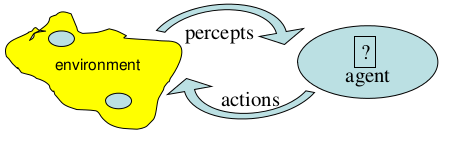
\includegraphics[width=0.6\textwidth]{img/mas.png}
	\caption{Basic multi agent system structure}
	\label{fig:mas}
\end{figure}

This allows the programmer to design proactive agents, which are set out to achieve ``well defined goals''. Agents' behaviours are thus goal directed. This requires the environment to be maintained in a certain state and the agent to achieve a certain state of its environment.~\cite{MAS-DoC}

From a software engineering perspective, the most adapted agent structure for our project is to use agents with states as shown in Figure~\ref{fig:agent-architecture}.

\begin{figure}[h!]
	\centering
	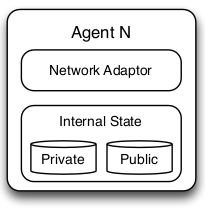
\includegraphics[]{img/agent-architecture.png}
	\caption{General agent architecture~\cite{Sam-Transfer-Report}}
	\label{fig:agent-architecture}
\end{figure}

We can use the agent's internal data to record information about the environment state and its history. Separating the internal state into public and private sectors also allows the agent to keep some information hidden from other querying agents. Finally, all \textsc{p2p} messages are sent via a network adapter which allows us to abstract away communication protocols and methods.

\subsubsection{Services and Protocols}

In order to simplify the implementation of agents, it was agreed that we would require additional services and protocols on top of the environment and network. Services allow us to retrieve the environment shared state raw data in a more user-friendly way. Similarly, protocols encapsulate inter-agent communication.

By using such components, we can encase the software implementation of our simulation framework. Any changes made to the way the environment stores data or how communications are handled would therefore not affect the behaviour of our agents.

\subsubsection{Presage2}

There exist several platforms that allow the development of multi agent systems. The two most important ones are Jade and Repast. However, it was decided to use the internally developed Presage 2 platform due to the nature of our desired simulation.

Originally written by Brendan Neville and then improved by Sam MacBeth, the platform offers the ability to rapidly prototype complex agent societies. In Presage 2, agents are allowed to act during incrementing time steps, which results in discrete time driven simulations. It also offers a rich communication layer as well as the ability to batch multiple simulation runs through a web user interface. Finally, the following requirements are met, which allow for the design of social behaviour and the observation of long term global performance and adaptation~\cite{Presage2-agent-societies}:

\begin{description}
	\item[Abstraction:] the agents and network can be as simple or complex as necessary (e.g.: agents can range from being simply reactive to implementing complex belief, desire and intentions (BDI).)

	\item[Flexibility:] the platform allows the user to easily change the simulation input parameters. In conjunction with the ability to batch run, it is very simple to measure the impact of variable values.

	\item[Extensibility:] base classes and modules can be extended in order to allow the user to add any desired functionality.

	\item[Interaction:] Simulation data can be stored in a MongoDB collection which provides easy access and visualisation of the results.

	\item[Rule engine:] There is support for executable, mutable rule specifications.
\end{description}

Figure~\ref{fig:presage2-architecture} and \ref{fig:presage2-lifecycle} respectively show Presage 2's general architecture and the breakdown of a simulation run:

\begin{figure}[h!]
	\centering
	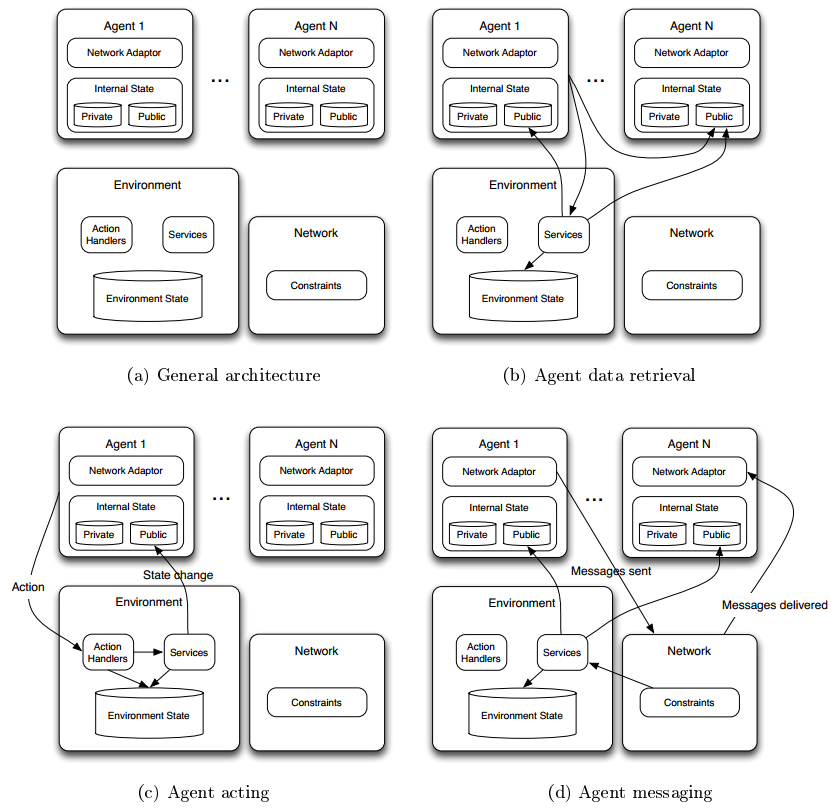
\includegraphics[width=\textwidth]{img/presage2-arch.png}
	\caption{Presage2 architecture~\cite{Sam-Transfer-Report}}
	\label{fig:presage2-architecture}
\end{figure}

\begin{figure}[h!]
	\centering
	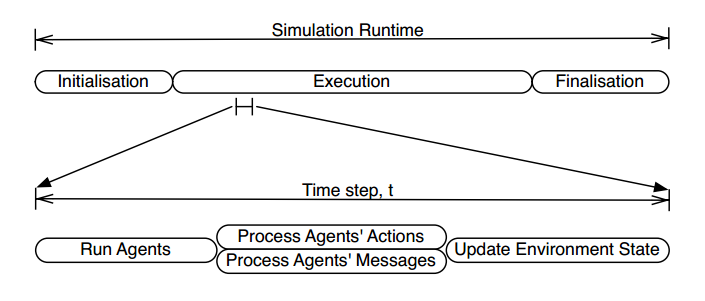
\includegraphics[width=\textwidth]{img/presage2-lifecycle.png}
	\caption{Presage2 simulation architecture~\cite{Sam-Transfer-Report}}
	\label{fig:presage2-lifecycle}
\end{figure}


\section{Defining our model}

This section details the design decisions made regarding the modelling of the Kyoto Protocol \textsc{cpr} system and its implementation as a multi agent system. We describe the simplifications made to the Protocol, and any assumptions about the real world and economy.

\subsection{Time}

With the understanding that Presage2 uses discrete time to run its simulations, we divided time into sessions, years, and ticks. Ticks map directly to Presage2's discrete units of time. Years last for a number of ticks defined at simulation time (defaulting to 365, which maps a single tick to a day in the real world). Sessions are composed of multiple years, with a default of 10. In the Kyoto Protocol, the length of a session is mutable depending on global economic and political climate. However, we felt it was a suitable abstraction from reality to use a consistent length for sessions throughout any individual simulation.

\subsection{Energy Output}

Energy output is the simplification of a participant's productivity. The calculation of a country's energy output depends on many economic factors, which would be too complex to accurately calculate for our model. We have simplified it such that it can be calculated using only two figures: the country's carbon output, and its fossil fuel percentage, that is, the percentage of the country's total energy that comes from fossil fuels. Using these two values, we can calculate the energy output, which is the amount of carbon the country would use if all of its energy was fossil-based:

\begin{center}
energy output = carbon output / fossil fuel \%
\end{center}

\subsection{Money}

Our model requires that participants have money to be able to spend on any of the actions available to them. Cash is thus calculated as a percentage of the participant's Gross Domestic Product (\textsc{gap}). Whilst in real life, countries may wish to vary their carbon reduction budgets, we decided that the percentage dedicated to green initiatives would remain constant.

\textsc{gdp} is initially set from real world country data, and it is understood that countries need to be able to affect their \textsc{gdp} rate (growth or contraction). In real life, \textsc{gdp} rates are controlled by a large number of factors; this has been simplified in our model such that \textsc{gdp} rate is only affected by energy output.

\subsection{The Kyoto Protocol}
The Kyoto Protocol can be summarised into the following flow of actions:

\begin{figure}[h!]
	\centering
	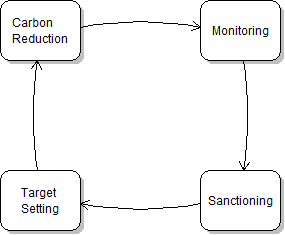
\includegraphics[width=0.3\textwidth]{img/Kyoto_4_states.png}
	\label{fig:kyoto_4_states}
\end{figure}

While we were eager to try and have our simulation model the Kyoto Protocol accurately, some changes needed to be made to discourage agents from abusing the game mechanics. For example, in a 10 year session, a participant could maximise their industry and \textsc{gdp} for the first 9 years and hence generate a large amount of fund. This could then be followed by a drastic reduction in industry to meet its target in the last year.

\begin{description}
	\item [Target Setting] \hfill \\ In the real world, targets are calculated per session for each participant. However, our model calculates the session targets for each participant, and then sets incremental, yearly targets which, if an individual country meets these targets, will ensure it meets its session target as well. This removes the potential abuse of the \textsc{gdp} functionality, since our simulated \textsc{gdp} is not externally sensitive to non-Kyoto Protocol events like \textsc{gdp} is in the real world.
	\item [Reporting] \hfill \\ Our model follows the Kyoto Protocol and reporting is done yearly.
	\item [Monitoring] \hfill \\ As per the \textsc{cpr} model, monitoring of participants should incur a cost. Every year all participants are 'taxed' a certain percentage of their \textsc{gdp} in our model, which is used to cover the cost of monitoring participants. The Kyoto Protocol does not specifically call for a tax to cover its monitoring, although the \textsc{unfccc} is funded by its members, so our model represents a suitable abstraction to reality.

In the real world, monitoring is done every 5 years by a team of experts. We decided to monitor more frequently in order to discourage unrealistic participant behaviour. A number of random participants are checked yearly using the funds gained from the 'monitor tax'. Repeat offenders, who have been found cheating before, have an increased probability of being monitored in the future.
	\item [Sanctioning] \hfill \\ Sanctions are applied immediately when participants are found to have missed targets or have reported fraudulent emissions. The sanction for missing a target is a proportional increase in that participant's target in the following year, which is in line with the Kyoto Protocol regulations.

The sanction for fraudulent reporting in real life are rather 'light weight', only suggesting a recalculation of the reported figures. In the real world, this kind of fraudulent activity would also result in political pressure from other Kyoto participants, but this would be hard to model in our simulation. We wanted to look at the effect of a more 'harsh' form of sanctioning, and thus it was decided to impose financial sanctions for fraudulent reporting.
\end{description}

\subsection{Participants \& Actions}
Countries which form part of the Kyoto Protocol have been split into 4 groups:

\begin{itemize}
	\item{Annex I (Must reduce emissions -- e.g. \textsc{eu})}
	\item{Annex I (Must sustain emissions -- e.g. Russia)}
	\item{Non-Annex I (Developing countries)}
	\item{Rogue Countries (Not part of Kyoto)}
\end{itemize}

While Annex I and Non-Annex I countries have been implemented as per the Protocol specification, it was decided that we would remove the Annex II class (which is just a subset of Annex I), and allow all Annex I classes to invest in \textsc{cdm}.

Table X defined the actions which participants can use:

%TABLE
\begin{center}
ADD TABLE HERE
\end{center}
%TABLE

\subsubsection{Domestic carbon reduction measures}
\begin{description}
	\item [Carbon Absorption] \hfill \\ Carbon absorption is the process of building carbon sinks, projects which offset carbon emissions, for example planting large sections of forest. As in real life, our carbon absorption model allows for diminishing returns, so as more carbon absorption actions are taken, the return received for a given investment decreases. This models the changes in land price after extensive forestation, and the increased difficulty of building further carbon sinks as more projects are constructed. In theory, the cheaper, more efficient projects are prioritized, so once they have been completed, greater investment is required for further improvement.

Our model only allows for forestation on arable land; this differs from real life where trees can be planted on various types of land. This simplification allows us to use freely accessible country data. Another simplification is the immediate building/growing of trees; in real life, a participant would only get gradual carbon reduction gains from planting trees. However, there are mechanisms in place within the Kyoto Protocol to immediately reward member states for sustainable development projects which reduce long term emissions. Our carbon absorption system models an abstraction of these two factors combined. 
	\item [Carbon Reduction] \hfill \\ Carbon reduction is the process of reducing carbon output of dirty industry. As in real life, our carbon reduction model allows for diminishing returns. Hence as more dirty industry is upgraded to clean one, the cost of further reduction increases. This maps to the ease of upgrading from coal power to existing, but cleaner natural gas technology, when compared to the investment required to pioneer nuclear fusion research.

Our model is only affected by the percentage of total dirty industry. In real life, there are various ways in which carbon reduction can be implemented, although the simplification used is suitable for the complexity of our model.
	\item [Energy Usage] \hfill \\ As previously described, participants need to be able to have some influence over their \textsc{gdp} rate. In our model, energy output is a driving factor behind the \textsc{gdp} rate calculations, and so participants have the option of either growing or constricting their industry. This has the effect of changing the energy output and carbon output accordingly.

Investments in carbon industry will result in \textsc{gdp} growth, capped at sensible levels, but increases in carbon emissions. Countries who must reduce their overall emissions but wish to still maximize their economic growth must first invest in carbon industry and then in carbon reduction or absorption.
\end{description}

\subsubsection{Flexibility Mechanisms}
\begin{description}
	\item [Emissions Trading] \hfill \\ In the real world, while being a viable carbon offsetting measure, carbon emission trading has proved less popular than domestic carbon reduction. Our model places more emphasis on emissions trading than in the real world, as we were interested in the simulation of an active commodities market.

It is understood that the world has several emission trading schemes and markets, the \textsc{eu ets} being one of the largest. While we did plan to incorporate the \textsc{eu ets} into our game, this was eventually scrapped as the time available did not warrant the extra complexity this would add to the simulation.
	\item [Clean Development Mechanisms] \hfill \\ \textsc{cdm} is a significant action available to participants of the Kyoto Protocol, and similar to our interest in an active carbon market, we were keen to see the effects of an active market for clean investment. This mechanism is broadly unchanged from the real world specification, with the exception that we are not differentiating between \textsc{aau}s and \textsc{car}s.
	\item [Joint Implementation] \hfill \\ The \textsc{ji} flexibility mechanism did not prove to be very popular in the real world, and with so few examples of this mechanism being carried out, it was left out of our simulation, and its inclusion would add unnecessary complexity.
\end{description}	
	
\subsection{Flowcharts}
Before moving to the coding phase of the project, some initial flow charts were drafted to help us visualise the different states and actions that would have to be implemented. The high level architecture of the simulation can be seen in Figure \ref{fig:kyoto_simulation_flowchart} with a more detailed composition of the country behaviour sub-process in Figure \ref{fig:country_behaviour_flowchart}:

\begin{figure}[h!]
	\centering
	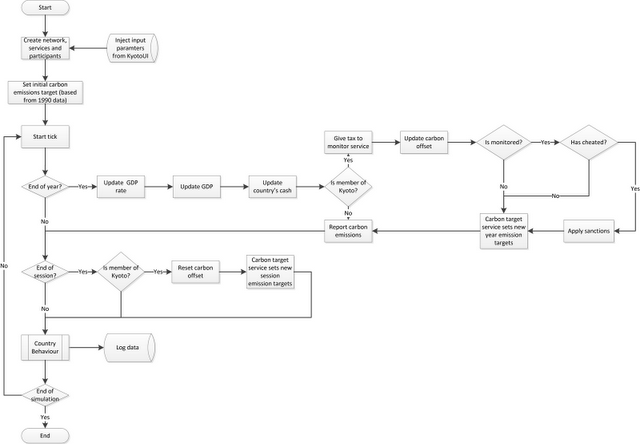
\includegraphics[width=0.8\textwidth]{img/kyoto_simulation_flowchart.png}
	\caption{Kyoto Simulation Flowchart}
	\label{fig:kyoto_simulation_flowchart}
\end{figure}

\begin{figure}[h!]
	\centering
	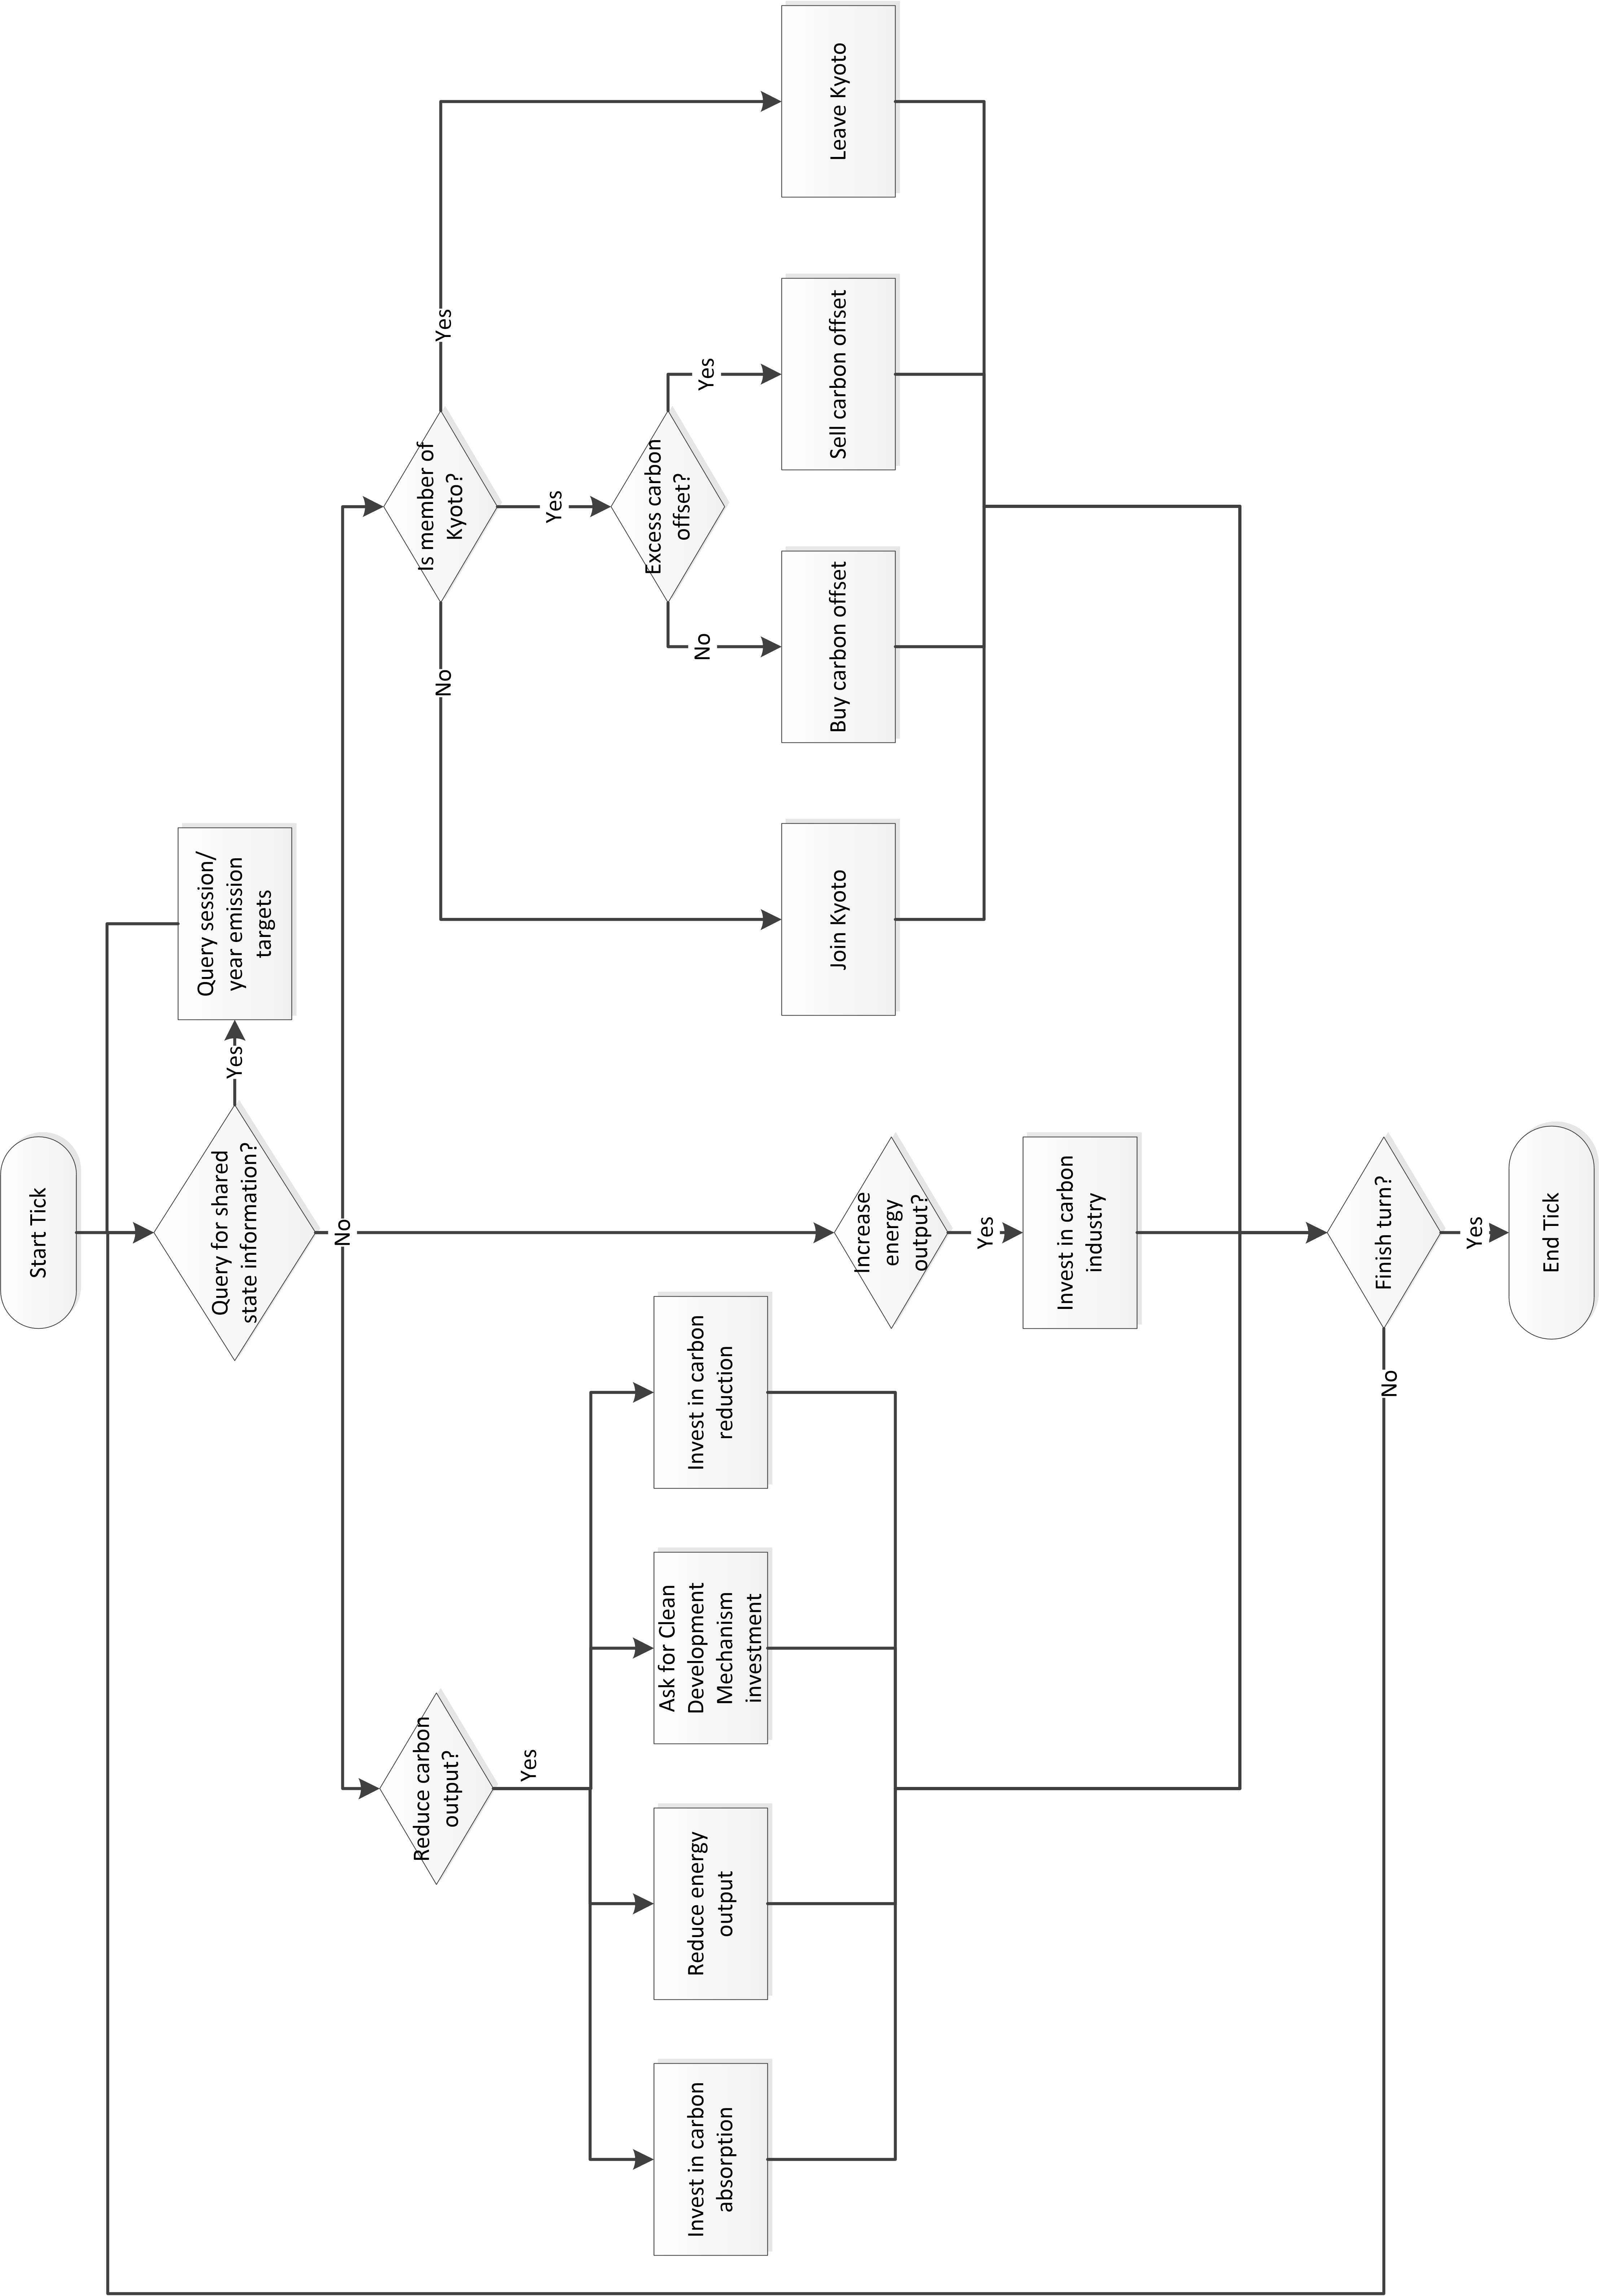
\includegraphics[width=0.8\textwidth]{img/country_behaviour_flowchart.png}
	\caption{Country Behaviour Flowchart}
	\label{fig:country_behaviour_flowchart}
\end{figure}


\section{Implementation}

\subsection{Agents}

%
% TODO
%

\subsubsection{Participants}

%
% TODO
%

\paragraph{Annex I (Sustain)}

Agents implementing this type of strategy are meant to represent countries which are part of Kyoto and belong to Annex I group, but their emission targets are equal or higher than their emissions for the first Kyoto session.

The usual reason for this is that normally, while the first session started in 1990, the data used for setting the targets comes from 1990. During this period of history, many Eastern Bloc countries moved from heavily carbon-based economies to more environmentally conscious economies. Hence, even though Kyoto takes their former high carbon emissions into account, they have reduced their carbon output quite significantly since then, reaching or even exceeding the targets before the first session started. That, in turn, means that they do not have to reduce their emissions further during the first session.

\subparagraph{Strategy}

In order to make strategies distinct between annex I sustain and annex I reduce, annex I sustain countries will only remain a part of the Kyoto Protocol as long as they meet their targets. In the event that emission targets are lower than the acceptable output level of an annex I sustain country, the country will depart from the Protocol and become a rogue state. 

However, it is important to recognise that annex I sustain countries did ratify the Kyoto Protocol when it was originally proposed and finalised. These countries' governments have expressed a desire to minimise their impact on the environment to some extent. It is with this in mind, that annex I sustain countries make sure that their overall emissions never rise above their starting levels. Any investment in industry to promote economic growth is offset by corresponding investments in cleaning industry or constructing carbon sinks.

On the other hand, annex I sustain countries are reluctant to reduce their carbon emissions if it adversely affects their economic growth. Any reductions in emissions are because the country has judged that investment will be profitable when the resulting offset is sold on the carbon commodity market. This may seem like a bleak attitude for a set of countries to adopt, painting them as opportunistic and self-interested. However, this diversified the strategies our countries employ over the course of an entire varied simulation and more properly models Common Pool Resources, where individual interests are weighed against that of the collective.

The strategy contains three steps, taken every year in order:

\begin{description}
	\item[1. Invest in industry] \hfill \\
	Part of a year's budget is reserved for increasing the economy. Since this group represents mostly newly-developed countries, this is prioritised to promote long term growth.

	As outlined earlier, the investment must be accompanied with carbon reduction or absorption, so that overall carbon emissions do not increase. To achieve that, a specific point is found for which total price of investments in industry and matching emission decrease is equal to the reserved budget.

	\item[2. Sell carbon credits] \hfill \\
	If the emissions of the country are lower than the target for a given year, the country will accumulate carbon offset, representing the `unused' emissions. The agents will attempt to sell all of these credits. Since carbon trading is essentially an open market, setting an average price can be challenging. To maximise profits from sales, the agents will start with a high asking price, reducing it gradually as the year progresses if no one is interested in buying, and increasing it when the sales go well.

	\item[3. Invest in emissions reduction] \hfill \\
	When a country has no credits to sell anymore, but there is still demand for carbon offset on the market, it may decide to invest in carbon reduction or absorption to generate additional carbon offset First, it estimates how many of the generated units can possibly be sold during the current session, assuming the market price persists. If the estimated profit is higher than cost of the investment, the country will proceed with it. Should this occur, the country will reduce its emissions by the end of the session (reducing global output as an incidental benefit), and hence will end up with a target higher than actual emissions in the next session, just as in the previous one. If this is the case, it will stay in Kyoto for the next session.
\end{description}

\paragraph{Annex I (Reduce)}

In our project, we define Annex I Reduce countries as participants whose current emissions are higher than their 1990 base targets, requiring them to prioritise the reduction of their carbon emissions. Good examples of such countries are the fifteen European countries.

For their behaviour, it was decided that the best approach was to design a mini simulation that would perform exhaustive testing on every possible country action, extrapolating emissions and industry growth into the future. It then decides which action results in the best outcome, with regard to maximizing economic growth while still meeting Kyoto Protocol targets and then performs the optimal actions in the simulation.

While simple in theory, in practice there are some major hurdles. The most troublesome of these is that there are an enormous number of possible actions a given Annex I Reduce country can take, all of which operate on a continuous scale. Every action has an almost infinite number of options that can be taken. For example, a country could choose to reduce their carbon emissions through absorption by spending 1\% of their available cash, or by spending 100\% of their available cash, or any number in between. They could then decide to buy vast amounts of carbon offset from the market, at any price, or put up sell offers. All of these actions can be performed in a single tick.

\subparagraph{Strategy}

Some heuristics had to be implemented to keep the simulation from spiralling out of control. It also ensured that as few \textsc{cpu} cycles as possible are wasted on actions that were simply irrational and could never lead to any useful results. To do this, it was decided to split each turn into three phases: the 'reduce' phase, the 'maintain' phase and the 'sell' phase.

The reduce phase happens first. It checks whether our current carbon output is below our carbon target. If we are at or below our target, then nothing is done. However, if we are above our current target, the testing will branch off into combinations of three distinct actions. The carbon target will be met by either buying carbon offset from the market, by reducing the carbon output through investing in absorption and reduction or, if in particularly dire financial situation, by reducing the economic output of the country. Every time a branch occurs, a new 'state' is created.

Before the maintain phase occurs, we compare every branched state with one another and check whether one state is objectively superior for every possible pair of states. For example, let a state have two attributes 'Money' and 'Carbon', where a higher 'Money' and a lower 'Carbon' is better. If state 1 has a 'Money' value of 100 and a 'Carbon' value of 50, and state 2 has a 'Money' value of 90 and a 'Carbon' value of 60, then state 1 is objectively better than state 2. Therefore we can immediately eliminate state 2 as a possible action. Alternatively, if a state 3 has a 'Money' value of 110 and a 'Carbon' value of 60, we cannot objectively say that it is any better than state 1 and thus cannot remove this from the simulation. By performing this culling, we can prevent our search space from getting too large and avoid going down paths where we can already tell there will be better alternatives.

Next is the maintain phase. As we are now guaranteed to be at least at or below our carbon target, the country can focus on improving its industry, which will eventually result in an increase in the available cash to spend. The simulation will branch off from each unculled state created in the reduce phase by first investing in industry (i.e.: increasing our energy output, which in turn increases our \textsc{gdp}) by some amount and then by offsetting the extra carbon created by investing in absorption and reduction, or by buying the offset from the market. Once again, a cull is performed after all branches have been taken.

Finally there is the sell stage. Here, we reduce our carbon output (by investing in carbon absorption and reduction, or by shutting down factories) by a certain amount and then sell our newly created carbon offset at the highest possible price. Once again, all unrealistic states are culled.

The combination of these three phases makes up a list of possible actions for one year of the game. However, since a session lasts a number of years (at which point any accumulated carbon offsets are abandoned when new emissions targets are calculated), simulating the possible behaviour for a single year simply does not provide us with enough information to choose an ideal action path. We need to continue the internal projections up until the end of the current session.

Once this is over and we have a large number of end states, we can analyse our them to find the ones which can be objectively considered the best. This will be the one with the best economy and the lowest carbon output. When identified, we simply traverse our path back to the initial state and perform the action path in the actual game.

Overall, this method takes full advantage of all possible options available to a country, including utilising the market as much as possible. No possible rational action is ruled out until it is clear that there are objectively superior alternatives. As a result, we achieve a behaviour that is very close to the optimal action for the country, resulting in maximum monetary gains while still reaching all set carbon targets.

As the annex I reduce countries were deemed to be paragons of justice, some actions such as cheating and ignoring carbon targets weren't coded in. However if a country finds itself constantly shutting down factories (due to a lack of money to perform any other actions) in order to meet carbon targets, it will choose to leave the Kyoto Protocol until it can get back on its feet again financially.

\paragraph{Non-Annex I}

The Non Annex I group is mainly composed of developing countries whose primary aim is economic growth. Since \textsc{gdp} growth is directly proportional to energy output in this project, the aim of Non Annex I countries is to increase its industry as much as possible. 

Investing in industry, and therefore growing a country's economy increases its carbon output at the same time. However, the Kyoto Protocol dictates that sanctions are not enforced on Non Annex I countries since they are not set targets to fulfill. They are therefore free to emit as much \CO as their industry requires.

Nevertheless, the Non Annex I behaviour was implemented such that they do care about the environment as well as their growth when cash is available in abundance.

The following keywords will be used to describe the general behaviour of Non Annex 1 countries:

\begin{description}
	\item[1. energy\_aim:] the energy output the country wants to reach by the end of the year.
	\item[2. times\_aim\_met:] how many consecutive times the energy output aim was met.
	\item[3. aim\_success:] variable that represents whether the country met its energy target or not.
	\item[4. green\_care:] variable that controls if the country cares or not about the environment.
	\item[5. green\_lands:] variable that controls whether the country has actually met its environmental commitments.
	\item[6. environment\_friendly\_target:] if it exists, variable that stores the country's carbon emission target. 
\end{description}

The country starts by having a policy of increasing its energy output as shown in Figure X whilst trying to meet an internally set carbon emission target.

\begin{align*}
	&times\_met\_before: \\
	&0 \rightarrow new\_energy\_aim = previous\_energy\_output + previous\_energy\_output / 8\\
	&1 \rightarrow new\_energy\_aim = previous\_energy\_output + previous\_energy\_output / 4\\
	&n \rightarrow new\_energy\_aim = previous\_energy\_output + previous\_energy\_output / 16exp(-0.693 \times n)\\
\end{align*}

Each year, the country calculates the difference between its achieved energy output and the target aim that was set the previous year. The difference is then used to estimate the amount of money to invest in carbon industry each tick in order to reach the required energy output. Before the country proceeds with the investment, certain conditions have to be met:

\begin{itemize}
	\item It has the available cash to spend.
	\item If the country has decided to care about the environment, the increase in carbon output due to the investment should not lead to its emission exceeding the set target.
\end{itemize}

If the latter condition is not met, then the country tries to invest in carbon absorption or carbon reduction in order to decrease its carbon emissions. However, the country will switch to non environmental friendly policies if it does not have enough money.
 
Non Annex I countries take part in Clean Development Mechanisms. This allows Annex I and Non Participant countries to invest in Non Annex I countries in exchange for carbon offset.

In other words, Annex I countries use Non Annex I land area and carbon output to reduce their own emissions in order to meet their targets in the Kyoto Protocol. There are two ways in which countries can invest:
 
\begin{description}
	\item[Carbon Absorption] Decrease available land area, increase carbon absorption
	\item[Carbon Reduction] Carbon output decreases
\end{description}
 
The amount of carbon output to be changed/given to the Annex I country depends on whether the Non Annex I countries meets its energy output aim.

Carbon absorption offers are all accepted if the country is in an environmentally friendly phase (unless the available land area is at a minimum). 

\subsubsection{Non-Participants}

For the purposes of our simulation the rogue states are comprised of the US and Canada, who operate independently of one another, yet necessarily share certain actions and behaviours. 

\subparagraph{United States}

The United States agent uses a metric of ``greenhouse gas intensity'', defined as the ratio of emissions to economic output, measured in units of tonnes of \CO per million dollars of \textsc{gdp} to monitor its emissions. For example, using the 1990 data values the simulation is seeded with the intensity evaluates to 4,879,376/5,722,300 = 0.853 (3dp). To put in historical perspective, the Bush administration committed to reduce the intensity of greenhouse gas emissions by 18\% over the period 2002-2012.

In the real world it is the governing political party that makes any decisions regarding climate change mitigation, whose actions are in theory in response to the prevailing attitudes of the electorate, and so it is the case for the agent in our simulation. Every four years an election is held, with the initial party in power chosen at random. For simplicity's sake only the two major parties of the republicans and the democrats are represented. Broadly speaking, the democrats seek to increase the intensity value being targeted (which will have a greater impact on carbon reduction), whilst the republicans will target higher growth rates. The ultimate goal of the governing party is to gain re-election, which, as will be detailed below, is determined by the reductions implemented and economic growth over the period. The degree to which each of these effects the re-election chances of the incumbent party varies according to the prevailing attitude of the electorate, and the party in question. The republicans are more strongly punished and rewarded for economic growth, whereas the democrats are more strongly influenced by their carbon reduction efforts (reflecting the concerns of their core supporters). 

The agent has three overarching behaviour patterns controlling its attitude toward carbon reduction, represented by a integer variable between 1 and 10, where 10 is highly positive, and 1 is ambivalent. The real world representation of this being the prevailing attitude of the electorate, to which, in theory, the governing party responds and chooses actions in accordance with. This attitude variable is specifiable at the beginning of the simulation, and can change year by year. A more positive attitude results in more ambitious targets for the desired intensity level improvement chosen for the election cycle. Additionally, the more positive the attitude, the more influenced by success or failure in reaching or exceeding reduction targets the populace are, and the less they are influenced by lower economic growth. The opposite is true for more ambivalent attitudes.

The agent, as in reality, is not a member of the Kyoto protocol at the start of the simulation, and thus is not subject to either monitoring or sanctioning. Despite its non-member status however, it is not entirely ambivalent toward carbon reduction. The agent has been designed so that through the natural oscillation of the party in power intensity levels will steadily decrease, and ultimately result in a decrease in absolute levels, which will result in the agent eventually joining the Kyoto protocol. Each year the agent checks to see if, were it part of Kyoto, would it have met its emission target. If for three years in a row the target is met then the agent joins Kyoto, conversely, if targets are not met for three years in a row after joining Kyoto, the agent will once again leave.

The winner of an election is decided by a function of the economic performance over the election cycle and the election year (the justification for the latter being the relatively short term memory of the typical voter), the carbon reduction measures undertaken, and the attitudes of the electorate and the party's core supporters toward these. After these factors have been taken into account, some level of randomness is introduced (perhaps one party has a particularly compelling candidate).

As the political party's re-election chances are determined by the levels of carbon reduction and economic growth achieved during the election cycle, it chooses targets for these (in the case of economic growth, assuming stable market conditions) in order to maximise this chance. The targets are initially based on the long term percentages reductions/growth rates achieved before being adjusted up or down. In order for an absolute decrease in emissions it is necessary for the emissions intensity to improve faster than economic growth. So, for an absolute decrease the targeted improvement in intensity must be higher than this. The desired improvement in the intensity level is thus taken at base to be the long term economic growth rate over the four year election period plus a value determined by the overall attitude of the electorate. E.g. If the year on year growth rate was 5\%, this would result in a 21.5\% compounded rate from the start to the end of the period. Targets are valid and acted upon over the four year election period in order to allow behaviors to adapt to the prevailing global economic conditions, in times where growth is strong, giving rise to more available cash, more investments toward carbon reduction are made, contrarily, during periods of poor economic growth more investments into the economy are made. 

Once the target is set, the agent sets about choosing actions. The agent aims to implement any actions over three years within the four year election cycle, allowing no action to be taken in one of the years if conditions are not favourable. If conditions are amenable, all available cash will be used. At the beginning of the election cycle the absolute carbon reduction required over the four year period (taking into account the expected \textsc{gdp} growth) is calculated. The goal in absolute terms for each of the three years is then set. The agent will attempt to fulfil its commitments during the first 99 ticks of the year (assuming a year is 100) through the clean development mechanism (\textsc{cdm}), or subsequent to Kyoto membership, through trading carbon offset with other agents. Before implementing any action, the agent evaluates whether the benefit to their election chances will be increased more by taking the action in question or an alternative. On the last tick of the year, if the targets for carbon reduction or \textsc{gdp} growth have not been met, then the agent will take appropriate action through the carbon reduction and absorption mechanisms, or through investing in industry. The party will take measures to meet either its reduction or growth targets first depending on, once again, the projected effect the meeting/not meeting one will have on their reelection chances. Then use any remaining cash available to meet (if possible) the remaining target. If both targets have been met, they will spend the remainder on their preferred action.

\subparagraph{Canada}

%
% TO BE FILLED OUT
%

\subsection{Participant actions}

\paragraph{Carbon handlers}

\subparagraph{Carbon reduction}

The cost of carbon reduction for a country depends on its ratio of carbon output to energy output, which can be described as a dirty industry percentage:

\begin{align*}
Dirty~Industry = Carbon Output~/~Energy Output
\end{align*}

The less dirty our industry is, the more expensive it gets to clean it further. Therefore, it is reasonable to use a measure of clean industry:

\begin{align*}
Clean~Industry = 1 - (Carbon Output~/~Energy~Output)
\end{align*}
 
The relationship between the cost of reducing carbon output by one unit and the percentage of 
clean industry at a given moment is given in Figure~\ref{fig:carbon_reduction}:

\begin{figure}[h!]
	\centering
	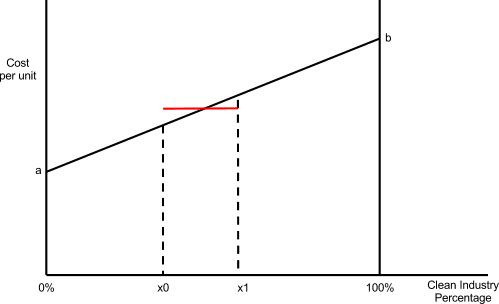
\includegraphics[width=0.6\textwidth]{img/carbon-reduction.png}
	\caption{Price of carbon reduction}
	\label{fig:carbon_reduction}
\end{figure}

Where:
\begin{itemize}
	\item a: cost of reducing carbon output by 1 with 0\% clean industry (min cost, constant)
	\item b: cost of reducing carbon output by 1 with 100\% clean industry (max cost, constant)
	\item x0: clean industry percentage before investment
	\item x1: clean industry percentage after investment
\end{itemize}

 
Hence, we can calculate cost of single unit investment at specific clean industry percentage using the following formula:

\begin{align*}
Unit~Cost = a + ((b - a) * x)
\end{align*}

Since the cost will increase linearly with every unit invested, we can find the average cost for the whole investment as the average of the initial and final cost (based on the x0 and x1 values). This is represented by the red line on Figure~\ref{fig:carbon_reduction}.
 
\begin{align*}
Average Cost &= ((a + ((b - a) * x1) - (a + ((b-a) * x0))) / 2 \\
&\Leftrightarrow Average  Cost = (a + ((b - a) * (x1 - x0))) / 2
\end{align*}

We can now calculate the total cost of a carbon reduction action by multiplying the average unit cost by the amount required by the country.

\subparagraph{Reduction cost estimate}

This `inverse' operation is mathematically solved with a quadratic equation. However, this is difficult to implement and is error-prone due to double arithmetic in Java. Instead, a binary search bounded between 0 and the current carbon output was used. In each iteration, the function calls the \texttt{getInvestmentRequired()} function with a hypothetical carbon reduction as parameter. It then adjusts the amount of reduction the country will receive depending on whether the returned value is higher or lower than the actual investment. Since there are 30 iterations, it will produce a an accurate result providing the current carbon output is less than 2$^{30}$.
  
This function allows participants to estimate and compare the profitability of a carbon reduction investment. As it is not used by the investment function itself, the lack of absolute accuracy is not crucial.

\subparagraph{Carbon Absorption}

The implementation of carbon absorption is very similar to that of carbon reduction investment. Here, the cost of forestation is inversely proportional to the percentage of area that is unoccupied with respect to entire land area of a country:

$$
Occupied~Area= 1 - Arable~Land~Area / Land~Area
$$

The cost of this action is calculated in the same way as for carbon reduction, with the only difference being the constant values for a and b. Additionally we also now need to calculate the area occupied by newly planted trees. This is done by using a constant specifying how much forest area is needed to absorb single unit of carbon, which is then multiplied by the amount of carbon absorption done.

\subparagraph{Absorption cost estimation}

Again, the implementation is the same as in the case of carbon reduction. There is only one difference, which causes a slight problem. Binary search requires lower and upper bound, and, potentially, carbon absorption can be as high as possible (providing a country has sufficient land and funds). Hence, we needed to use some upper bound to allow using binary search algorithm.

Even though a country can invest in carbon absorption as much as it wants, it does not make much sense for it to exceed carbon output, and shouldn't be realistically possible providing reasonable constants for prices. Hence, the upper bound which is used here is a difference between carbon output and carbon absorption of a country, so that, for maximum investment, the function will return absorption change which forces actual emissions to atmosphere to 0.

Still, this will produce false results where investment is high enough to potentially increase carbon absorption beyond carbon output. Again, this is just an additional function for countries to make writing strategies easier and make them more interesting. Since there is no way around it, it was decided to allow this potential inaccuracy.

\paragraph{Energy handlers}

Each country in our simulation has the ability to influence its economy by investing or reducing its carbon industry. This functionality is provided to each participant through an instance of the energy handler. Unlike the carbon handlers, the price of a unit of investment in your carbon industry is a constant defined at the start of the simulation. In addition, there is no cap on the amount a country is allowed to develop its industry. 

The cost of an investment for a given desired growth can be modelled by the following linear function:

$$
Cost = Growth \times Price~of~Carbon~Investment
$$

Similarly, each participant can also use the handler to query how much economic growth can be achieved for a given cost:

$$
Growth = Cost / Price~of~Carbon~Investment
$$

Using these two functions, participants can make an informed decision on whether to invest in their industries or decide to reduce it. A country can increase its \textsc{gdp} by building factories which in turn will give them more money to spend in the following year. However, its carbon emissions will also increase as a result.

On the other hand, a country can decide to close down factories. This is a cost free method of reducing carbon emissions, though it also leads to a contraction of its economy and \textsc{gdp}. 

\paragraph{Carbon reporting}

%
% TODO: NEEDS CONTENT
%

\paragraph{Joining \& Leaving Kyoto}

In our simulation platform, we allow countries to leave and join the Protocol. In order to replicate the Kyoto country categories, it was decided to offer participants three distinct levels of subscription to the simulation using Java enumerated states. Each of these give access to a different set of possible actions as described previously. Using this functionality, we can emulate real world scenarios such as Canada leaving the Protocol.

\subsection{Protocols}

\subsubsection{Trade Protocol}

The Trade Protocol allows participants to engage in trading of carbon offset or Clean Development Mechanism (\textsc{cdm}) investments in other participants/countries. The Trade Protocol class inherits from the \texttt{FSMProtocol} class provided in the Presage2 \textsc{api}, which is an implementation of agent protocols, used by agents to communicate with one another.
 
The trade protocol can be used for both carbon trading and Clean Development Mechanisms. The type of message that the trade protocol deals with is an object of type \texttt{OfferMessage}. The \texttt{OfferMessage} object has information of who initiated the conversation and who broadcast the offer in the first place and all the information about the quantity and unit cost of the offer. The quantity refers to the total, in tons of carbon offset, that are being offered. The unit cost refers to the price per ton. The total cost of the offer is the product of these two values.

When a participant broadcasts a carbon trading offer then the type of the Offer (also another 
object that \texttt{OfferMessage} encapsulates) is set to either:
 
\begin{itemize}
	\item \texttt{BUY}: If participant wants to buy carbon offset.
	\item \texttt{SELL}: If participant wants to sell carbon offset.
\end{itemize}

For Clean Development Mechanisms, the trade protocol allows the participant to advertise whether they want other countries to invest in their industry to reduce carbon emissions. When a participant wants to advertise about CDM then the following types need to be assigned to the \texttt{OfferMessage} Offer type:

\begin{itemize}
	\item \texttt{INVEST}: participant wants to invest in another country.
	\item \texttt{RECEIVE}: participant is asking for other countries to invest in their industry/country.
\end{itemize}

It is also further specified whether the form of \textsc{cdm} is for carbon reduction or carbon absorption, which restricts the participant to choose the following investment types:

\begin{itemize}
	\item \texttt{ABSORB}: Whether the investment will be used to reduce carbon emissions by investing in absorption techniques.
	\item \texttt{REDUCE}: Whether the investment will be used to reducing carbon emissions via investing in carbon reduction techniques.
	\item \texttt{INVALID}: If investment type does not exists as it is a buy or sell carbon offer.
\end{itemize}

\paragraph{Functionality}

Trade Protocol works in the following ways:

\begin{enumerate}
	\item A participant who is willing to engage in a trade sends a broadcast message using the \texttt{network} object provided to every agent. This message contains information about the trade as they wish it be carried out.
	\item Another participant who is interested in the offer broadcasted can start a protocol conversation with the broadcaster. They can reply with slightly altered offers, to simulate a minor form of negotiation.
	\item The broadcaster can then accept or reject the offer that is proposed by the initiator.
\end{enumerate}

The process is better illustrated with the following diagrams:

\begin{figure}[h!]
	\centering
	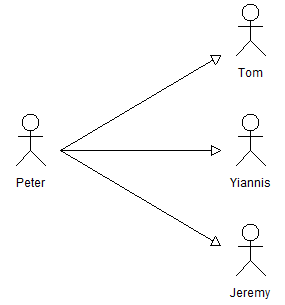
\includegraphics[width=0.4\textwidth]{img/protocol1.png}
	\caption{Broadcaster multicasts a message to other agents}
	\label{fig:protocol1}
\end{figure}

Other agents will receive the offer message and can choose to start a \texttt{TradeProtocolFSM} conversation with the broadcaster.

\begin{figure}[h!]
	\centering
	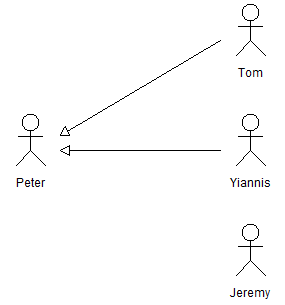
\includegraphics[width=0.4\textwidth]{img/protocol2.png}
	\caption{Tom and Yiannis wishes to respond to the broadcast message}
	\label{fig:protocol2}
\end{figure}

In this example, only Tom and Yiannis decided to respond to the broadcast message sent by Peter.

\begin{figure}[h!]
	\centering
	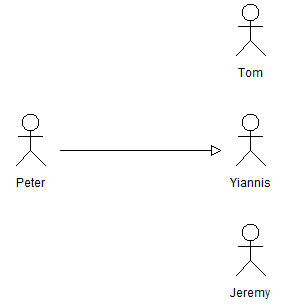
\includegraphics[width=0.4\textwidth]{img/protocol3.png}
	\caption{Peter decides to respond}
	\label{fig:protocol3}
\end{figure}

Agent Peter can then decide whom to finish the trade with. In this case he decides to accept the offer initiated by Yiannis.

\paragraph{Reverting}

In the event that a trade is unable to be carried through to the end, possibly caused by one of the countries not having enough available funds to complete the transaction, the trade can be reverted, and the involved parties are refunded.

\paragraph{Trade Protocol state machine}

The protocol has two different state machines that are used by the initiator and the broadcaster. The state machines are as follows: 

\begin{figure}[h!]
	\centering
	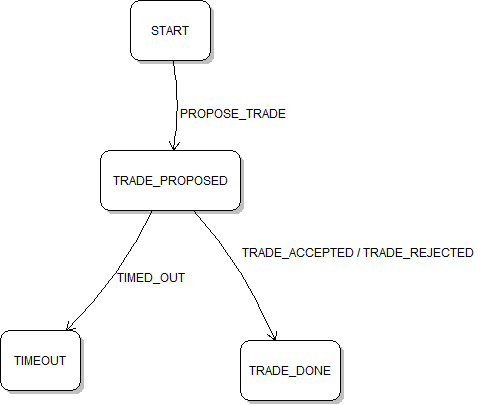
\includegraphics[width=0.6\textwidth]{img/protocol-fsm-1.png}
	\caption{Initiator \textsc{fsm}}
	\label{fig:protocol-fsm-1}
\end{figure}

\begin{figure}[h!]
	\centering
	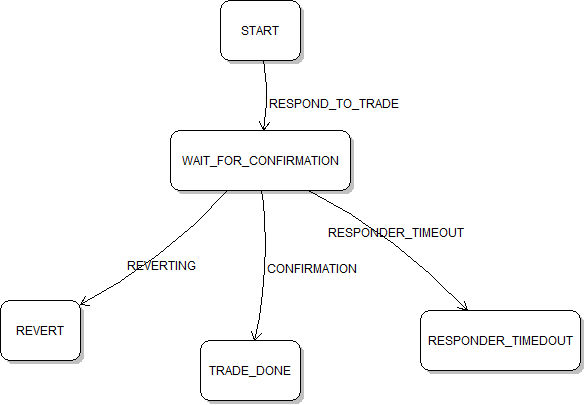
\includegraphics[width=0.6\textwidth]{img/protocol-fsm-2.png}
	\caption{responder \textsc{fsm}}
	\label{fig:protocol-fsm-2}
\end{figure}

Figure-X and figure-X shows the state machines used by the Initiator and Responder respectively along with the transitions labelled on the arrows. The transitions in an \texttt{FSMProtocol} happen when a participant receives a message.

\paragraph{Initiator FSM}

Both the initiator and the responder have a single \texttt{START} state as required by the \texttt{FSMProtocol}. The initiator has two end states, which are \texttt{TIMEOUT} and \texttt{TRADE\_DONE}. Each transition results in the participant performing a particular action of sending back a message to the responder, which makes the responder transit to the next state.

\begin{description}
	\item[1. \texttt{PROPOSE\_TRADE}:]
	When the participant responds to the offer, it transitions to the \texttt{TRADE\_PROPOSED} state and sends a Unicast message to the broadcaster waiting for its response.
	\item[2. \texttt{TIMED\_OUT}:]
	From the \texttt{TRADE\_PROPOSED} state a timeout of 3 ticks is set so that the initiator times out into an error state.
	\item[3. \texttt{TRADE\_ACCEPTED}:]
	If the responder accepts the trade proposal, the Trade Protocol handles the trade completion through a function called \texttt{handleTradeCompletion()}. If anything goes wrong while handling the trade completion then the participant (initiator) transits to the \texttt{TRADE\_DONE} state by sending a Unicast message to the responder to revert the changes. If the handling of trade completion works well then the participant transitions to the end state \texttt{TRADE\_DONE} by sending a confirmation message to the responder.
	\item[4. \texttt{TRADE\_REJECTED}:]
	If the trade was rejected by the responder then the participant (initiator) transits to the \texttt{TRADE\_DONE} state by sending a confirmation unicast message to the responder that it has received the message.
\end{description}

\paragraph{Responder FSM}
 
Figure-X shows the \textsc{fsm} that is used by the responder. Upon receiving a message form the initiator. There is only one \texttt{START} state and the three end states are \texttt{REVERT}, \texttt{TRADE\_DONE} and \texttt{RESPONDER\_TIMEOUT}. Similar to the initiator, the transitions happen with the participant sending a unicast message to the initiator agent.
 
\begin{description}
	\item[1. \texttt{RESPOND\_TO\_TRADE}:]
	This transition occurs when the initiator spawns a message, which makes the responder transition to the \texttt{WAIT\_FOR\_CONFIRMATION} state. If the responder accepts the exchange then it transitions to the next state by sending a unicast message to the initiator that it accepted the trade, otherwise it transitions to the next state by sending a unicast message to the initiator that it has rejected the offer. Once the participant makes the decision to accept the offer then the \texttt{handleTradeCompletion()} function is called to adjust the carbon offset and cash of the responder. If things fail for reasons such as not enough cash exception from the responder then the changes made to the responder’s carbon offset and available to spend will be reverted. Nevertheless, a reject message is sent to the initiator to inform him that the trade was unsuccessful.
	\item[2. \texttt{REVERTING}:]
	If the initiator fails in completing the trade for reasons such as not enough cash exceptions, then the initiator reverts itself and sends a message to the responder. Once the responder receives this message then it goes to the \texttt{REVERT} state via the \texttt{REVERTING} transition. There, it reverts all of the changes since the start of the conversation.
	\item[3. \texttt{CONFIRMATION}:]
	This is a transition to from \texttt{WAIT\_FOR\_CONFIRMATION} to the end state \texttt{TRADE\_DONE} state. This transition happens when either trade was successful or was unsuccessful (i.e. the responder rejected the trade in the first place).
	\item[4. \texttt{RESPONDER\_TIMEOUT}:]
	Timeout condition of 3 ticks from \texttt{WAIT\_FOR\_CONFIRMATION} state to the \texttt{RESPONDER\_TIMEDOUT} state, which is the end and error state of the responder.
\end{description}

\subsubsection{Time Service}

The time service is an environment service, extending Presage2's existing environment interaction classes and development framework. It allows for coordination of time-based events and synchronises various features within our Kyoto Protocol simulation. Although Presage2 does have existing objects (SimTime) which can be used to attain simulation time, this is an absolute value in discrete logical time since the beginning of the simulation. It therefore does not take into consideration the variety of chronological distinctions the Kyoto Protocol requires, such as subdivisions into years and sessions.

It was initially decided to use a global service. It would perform most of the logic integral to coordinating time-driven activities, and would be layered on top of Presage2's integrated SimTime object. However, it is necessary for agents to be able to query for information regarding the current year and session in order to make important strategic and behavioural decisions. Presage2 enforces that agents (participants) are unable to communicate directly with global services. While agents can act on the environment and affect services, performing the reverse is somewhat more complex.

At this stage, it would seem a participant time service would be more appropriate, since participant services can communicate directly with agents. However, another key functionality of the time service is the publishing of new events, both for the end of years and sessions, which trigger key monitoring, sanctioning, reporting, and architectural actions essential to the managed nature of the Kyoto Protocol. Unfortunately, implementation is not in place within Presage2 for participant services to generate (or interact with) the EventBus class, the object essential to publishing or receiving events.

With these restrictions in mind, the time service was subdivided into two separate services. The participant service communicates with agents and relays information regarding the current year and session, among other minor time-related information gathering tasks. The global service is the backbone of the time service, generating new year and session events for the monitoring and targeting services to hook onto. It also carries out calculations to derive the current year and session from the discrete simulation time and communicates this information to the participant service.

Both classes extend from Presage2's predefined EnvironmentService class, and use Google's Guice injection systems for initialisation and, in the global service's case, to register with the EventBus.

\subsubsection{Monitor}

The monitor's purpose is to regularly check whether countries are meeting their targets and randomly check for false carbon emission reports. If either case is true, a scaling sanction is applied to the country.

We were initially unsure whether the monitor should be an independent agent or an environment service. We settled on making it a service, so that it could listen to an event that would trigger the monitoring as agent are unable to do so.

When countries are initialised they subscribe to the monitor either as Annex I or Non Annex I. Although only Annex I countries are monitored, the Non-Annex I countries list was required to fix an issue with events at the end of a year happening in the right order. Indeed, countries were calling for their targets for the next year to be updated before the monitor could compare the results for the previous year against its previous targets. This was fixed by updating targets after the monitoring function in the Monitor service.

Every year the monitor charges the Annex I countries a tax, which is used to perform the monitoring action on randomly selected countries. If the monitor runs out of money, it cannot monitor and countries are free to behave without fear of sanction (although this information is hidden).

\subsubsection{Carbon Target}

The carbon target service is responsible for reducing the world carbon emissions through the calculation of targets for all Annex I Kyoto members. Within the Presage2 simulation it is set up as a global service, this enables it to listen on an event bus and run independently from the country agents.
 
All target calculations are triggered by the end of year event generated by the time service via a method call from monitor.

\paragraph{How targets are calculated}
\subparagraph{For the whole world:}
Reduction Coefficient = 0.95 (5\% reduction)
s = current session number
World session target [s] = world session target [s - 1] * Reduction Coefficient
Kyoto target [s] = world session target [s] - total non annex I output [s - 1]

\subparagraph{For Annex I countries:}
\subparagraph{Each Session:}
y = current year number
Country Proportion [s] = country output [y - 1] / (world output [y - 1] - non annex I output [y - 1])
Country Session Target [s] = Kyoto target [s] * country proportion [s]
 
\subparagraph{Each Year:}
Session Progress = current year in session / number of years in session
Session Target Difference = session target [s - 1] - session target [s]
Year Target = session target[s - 1] - session target difference * session progress - penalty

In the event that a session target is needed from before session 0, world data from 1990 is used in its place. This models the Kyoto Protocol's basis of its initial targets.
 
To avoid unfairness and promote economically feasible targets, as is negotiated in the real Kyoto Protocol, we restricted the maximum reduction across a single session to be 10\% of total emissions. Without this limitation, large emissions from rogue states can cause targets for annex I targets to reduce unreasonably quickly. To handle unusual corner cases that may cause a country's session target to be higher than its previous session target (possibly due to drastic reductions by other member states, or large emissions from rogue states) we have restricted session targets so they cannot have a higher value than the previous session target.
 
Non annex I countries are not calculated a target. However, both non Annex I countries and rogue states have an impact of target assignment. As can be seen in the above formulas and in keeping with the objects of the Kyoto Protocol in reality, the aim for a single session is to reduce global \CO emissions by 5\%. After calculating the desired output for this session, the targeting service calculates the required reduction from member states, assuming non Annex I countries and rogue states continue producing the same amounts of \CO.

\paragraph{Implementation}

The carbon target service retains all the necessary data required for the above calculations in a private arraylist. Year targets are also set using a package protected method in the \texttt{AbstractCountry} superclass.
 
Within our simulation it is possible for countries to report false carbon emissions. Each year monitor service decides to monitor a subset of the countries. If a country is found to have reported a false value, its \texttt{UUID} is added to a list of cheaters. This list is then passed to \texttt{CarbonTarget} each year by \texttt{Monitor}, and is referenced when querying carbon output values for the target calculation.
 
Some countries (for example the \textsc{us}) may wish to join Kyoto at some point during the simulation. Since individual year targets are interpolated values dependent on session targets, and session targets are dependent on global emissions and each country's status as a rogue or member state, having a country join the Kyoto Protocol mid session is, in our simulation, extremely difficult. Each country's target would need to be recalculated and this introduces potential conflicts with existing strategies that the member state AIs have chosen. As a solution to this, we decided that rogue states could only join Kyoto at the beginning of a new session. Any rogue state that attempts to join the Kyoto Protocol in the middle of a session will be put on a waiting queue and will automatically be registered and become an Annex I country at the beginning of the next session.

We decided that any rogue state joining the Kyoto Protocol would automatically become an Annex I country for two reasons. One was the simplification of the rejoining process, which had already become extremely complex. Also, when compared to reality, it seemed reasonable that any country which left the Kyoto Protocol and then rejoined at a later date would then be assigned targets and monitored, to ensure that the system was not abused for financial gain. The US, the only major nation that did not ratify the Kyoto Protocol at its inception, would be an Annex I country regardless, were it to participate.

Leaving Kyoto is another potential action taken by member states, as seen in reality when Canada departed the Kyoto Protocol in 2011. When a member state leaves, its output is immediately recognised as that of a rogue state, and its departure has an effect on the setting of new session targets after the current session ends.   
 
Joining and leaving the Kyoto Protocol, as well as other actions such as reporting \CO emissions to the monitoring service, are implemented via action handlers, integrating with Presage2's defined structure for agents communicating with non-participant services and the multi-agent systems design paradigms regarding agent interaction with the environment.

\subsubsection{Market}

Our Kyoto simulation integrates a very basic emulation of the state of the financial markets. Each year, the market state will be determined randomly and affects by how much a country's \textsc{gdp} will change. By default, there is a 10\% probability that the economy is stable, 10\% that it is in recession and a 80\% probability that it is in a period of growth, but these can be changed by the user when running a new simulation.

\subsection{Game Balancing}

As we have seen, the game is made up of a series of mathematical functions, many of which rely on a set of constants (eg. \texttt{GROWTH\_SCALAR}, \texttt{MAX\_GDP\_GROWTH}). Varying and balancing these constants allows us to create varied and accurate simulations. These can be either initialised at compile time, or injected by the Kyoto \textsc{ui} at runtime, in order to run a wide range of different scenarios.

The balancing of these constants was not a simple task, since changing one may have an impact on others. The following 3 facts were used as a starting point for calculating suitable values for some of the constants:

\begin{enumerate}
\item Each country has an emission target of -5\% from their base year.
\item Countries typically invest 0.5\% of their \textsc{gdp} in developing clean industry every year.\cite[Figure 12]{PEW-Environment}
\item It takes ~0.0156 km$^{2}$ of trees per tonne of carbon absorbed.\cite[Accessed Jun 2012]{Trees-in-Trust}
\end{enumerate}
  
From 1, we can derive: 

\begin{enumerate}[resume]
\item The likely energy change per year (~ 0.05%)
\item \textsc{gdp} rate, since we can work out the energy difference
\end{enumerate}

From 2, we can derive:

\begin{enumerate}[resume]
\item The amount of cash each country gets each year
\item Sanction rate and tax rate as proportion of cash
\end{enumerate}

From 4 and 6, we can derive:

\begin{enumerate}[resume]
\item The cost of carbon reduction and absorption.
\end{enumerate}

\subsection{Kyoto UI}

\subsubsection{Overview}

The Kyoto \textsc{ui} is a web interface designed for instantiating and editing Presage 2 simulations. Web technologies used include an Apache web server, \textsc{php}, \textsc{html} and Javascript. Combined with a few additional libraries, these technologies provide the functionality required to display rich pages which allow for good visual representation and easy editing of data.

\subsubsection{Database Implementation}

The mongo database is interfaced using an \textsc{odm} (Object Document Mapper) library called mongorecord. This wraps interfaces for querying and writing the collections in the database with \textsc{php} classes which can be instantiated and used throughout the project.

\subsubsection{Simulation Initialisation Data Import and Export}

In order for any simulation to have a starting point, data must be imported containing information such as how long the simulation should run for and the data is required to set up each of the agents. Presage 2 has a command line interface which can be used to create simulations in the database and add parameters to them. The structure of these simulations in the database was used as a framework to import \textsc{csv} files of data to create simulations in the same format as generated by the Presage 2 \textsc{cli}.

\subsubsection{CSV Import and Export Functionality}

To get data in and out of the system \textsc{csv} (Comma Separated Value) files are used. This is a convenient method of transferring data as the \textsc{csv} file can be opened and edited in spreadsheet software such as Microsoft Excel. Data collected on countries of the world is inserted into the simulations, as are parameters from 'default' \textsc{csv} files. Once these are in the database, the \textsc{ui} can copy and edit them. Simulations can then be exported as a backup or to transfer them to another database. This functionality underpins the whole simulation by providing an easy way to get a huge amount of data in and out of the system quickly, easily and reliably.

\subsubsection{Simulation Editor UI}

Once data has been imported from the \textsc{csv} file it may be necessary to make new simulations by changing parameters etc. This is one of the main tasks of the web \textsc{ui}, to make this editing visually comprehensive and easier than manually editing the \textsc{csv} file or the database entry.

\subsubsection{Agent (Country) Data}

Most agents in the simulation are countries and in order for the simulation to be as realistic as possible these are modelled on real countries with parameters describing land mass etc. stored in the database. It is useful to edit some of these parameters such as the percentage of land mass available for green development to investigate what happens in a simulation given agents with different parameters. In the \textsc{ui} there is a page specifically for editing countries which displays a clickable map of the world with a dropdown menu for country selection. This way all countries within a single simulation can be displayed as a bunch of editable parameters.

% UI IMAGE

\subsubsection{Simulation Data}

Once imported, simulation data resides in a collection in the database. The \textsc{ui} provides a list of all simulations stored in the database with some basic information about the simulation displayed in the list. Next to each simulation is a menu which allows you to do several things with the simulation: view (detailed view of the simulation in the database),  export the simulation as a \textsc{csv} file, edit the simulation, copy it, or delete it.

\paragraph{Simulation Overview Page}

% UI IMAGE

The simulation overview page displays a world map using colour to indicate the values of a selected parameter for each country (default is arable land area percentage). There is a drop down menu (called Map View) which allows changing of the parameters displayed on the map. Below this is a table displaying a detailed output of all the simulation data from the database. This page also links to the \textsc{csv} export feature, copy feature, edit simulation page and a dropdown is present to allow editing of all the countries within the simulation.

\paragraph{Simulation Edit Page}

% UI IMAGE
 
The simulation edit page is a low level editor for the simulation. Functionality is provided to rename the simulation, the simulation authors and all other simulation attributes which it makes sense to edit. It also provides a link to the country editor page (the simulation \textsc{id} is passed in the \textsc{url} to ensure editing takes place on the countries of the correct simulation).

\paragraph{Simulation Results} % The displaying of

%
% TODO: Write about this
%


\section{Results}

%
%	Introduction here
%

\subsection{Scenarios}

The outcomes and agent activity of any individual simulation can be influenced by... 

\begin{description}
\item[Session Length] \hfill \\

Session length refers to the number of years in a given commitment period. The longer the sessions, the longer countries will have to meet their target. If this is set too short, countries will be more likely to miss their targets or cheat. This will have repercussions on their ability to spend and invest. They may also choose to just leave the protocol altogether.

\item[Monitor Price] \hfill \\

This is the price to monitor each country every year. This has been chosen to allow fewer countries than there are in the simulation to be monitored. We were aiming for approximately 10\% of cheating countries to be caught. This was to emulate a more realistic situation where monitoring everyone is not possible. However we didn't want to set the price too high, or cheating might become the optimal behaviour.

\item[Investment in Industry] \hfill \\

This will effect how large an increase in \textsc{gdp} rate countries will see for a given investment. If this is too low, it would take too long for countries to see any benefit, and they would prefer to hang on to their money. Too large, and it would become unrealistically easy to meet targets without trading.

\item[Disabling Monitoring] \hfill \\

This could be achieved by setting the monitor tax to 0. Although our behaviours make little use of cheating, disabling the monitor would yield interesting results in a more realistic simulation. Giving countries free reign over meeting their carbon targets would be a test of the morality in their behaviour (if any). The likely result would be no targets being met and global carbon emissions increasing.

\item[Participants] \hfill \\

Removing the so called `rogue' countries (\textsc{us}) from our simulation would have a large beneficial effect on global emission  targets for the remaining participants. This scenario could be compared to a real-world situation where these countries' outputs don't contribute to the way Kyoto set its targets. Although this probably wouldn't help the global carbon emission problem, countries would be more likely to stay if their targets were easier (see Canada).

On the other hand, we could simulate only having 'rogue' countries who behave only according to their own internally-set targets. The resulting behaviour would probably be chaotic and not beneficial to the global emission problem. This would be similar to the possible real-world situation where all countries withdraw their support for Kyoto, but commit to their own reduction targets.

The last hypothetical situation we thought would be of interest was if all countries ratified and were classified as Annex 1. Emission targets would be much simpler to understand (and fairer compared to the \textsc{us}'s current unrattified status). Also no \textsc{cdm} would take place. This would take away one of the easiest ways for a country to meet their targets while keeping their heavy carbon industry. There is much concern in the real world over the effectiveness and morality of using \textsc{cdm} to reduce carbon emissions. Taking away arable land from third world countries that could be used to grow crops, just to plant trees which will take several decades to become effective carbon sinks sounds very dubious.

\item[CO$_2$ Reduction Rate] \hfill \\

The faster countries have to reduce their carbon, the more likely they are to miss their target, cheat and/or leave the protocol. We predict a lower reduction rate would be the most beneficial in the long term.

\item[GDP Investment] \hfill \\

Realistically, will invest a different proportion of \textsc{gdp} into clean initiatives. Due to countries not needing to worry about spending money on anything non-Kyoto related in our system, we set a fixed percentage to be invested in clean initiatives and industry expansion. If this parameter is high, countries will have plenty of money to invest in their own industry and international projects, so targets will be much easier to meet. The opposite would make each move more valuable and although targets would be harder to meet, countries may make 'wiser' decisions.

\item[GDP Growth] \hfill \\

We have enforced an upper and lower limit on \textsc{gdp} growth of $\pm$-7\%. This reflects the typical real-world values for the majority of stable countries. Increasing this range would make the market more volatile. During growth, investment in industry will have an exaggerated effect, whereas global recession could make it difficult for anyone to meet their targets.

\item[Market State Factors] \hfill \\

These effect the chances of the global economy being in recession or growth, with a weighting towards remaining stable. These could be varies to emulate the protocol during an extended period of either negative or positive growth. The effects would be very similar to changing the \textsc{gdp} growth range as above.
\end{description}


\bibliography{report}
\bibliographystyle{references}

\end{document}
